\documentclass[11pt]{article}

\usepackage[left=1in,right=1in,top=0.70in,bottom=0.70in]{geometry}
\usepackage[utf8]{inputenc}
\usepackage[T1]{fontenc}
\usepackage{lmodern}
\usepackage{microtype}
\usepackage{graphicx}
\usepackage{booktabs}
\usepackage{amsmath}
\usepackage{amssymb}
\usepackage{algorithm}
\usepackage[noend]{algpseudocode}
\usepackage{caption}
\usepackage{subcaption}
\usepackage[most]{tcolorbox}
\usepackage[numbers,sort&compress]{natbib}
\usepackage{xcolor}
\usepackage[colorlinks=true,allcolors=blue!55!black]{hyperref}
\definecolor{originblue}{HTML}{123E6D}

\graphicspath{{used_pngs/}}
\captionsetup{font=small,labelfont=bf,skip=7pt}
\linespread{1.06}
\setlength{\parindent}{1.4em}
\setlength{\parskip}{0.70em plus 0.1em minus 0.1em}
\setlength{\textfloatsep}{15pt plus 3pt minus 2pt}
\setlength{\intextsep}{13pt plus 2pt minus 2pt}

% Let floats fill pages rather than leaving a gap when a figure jumps.
\renewcommand{\topfraction}{0.92}
\renewcommand{\bottomfraction}{0.85}
\renewcommand{\textfraction}{0.06}
\renewcommand{\floatpagefraction}{0.80}
\setcounter{topnumber}{4}
\setcounter{bottomnumber}{3}
\setcounter{totalnumber}{6}

\begin{document}

\begin{tcolorbox}[
  enhanced,
  colback=white,
  colframe=originblue,
  boxrule=0.7pt,
  arc=9pt,
  outer arc=9pt,
  left=16pt,
  right=16pt,
  top=14pt,
  bottom=12pt,
  before skip=0pt,
  after skip=15pt
]
\begingroup
\setlength{\parindent}{0pt}
{\raggedright\color{originblue}\fontsize{18}{21}\selectfont\bfseries
Astra: Histology-Derived Single-Cell Spatial Transcriptomics for Clinical
Prediction\par}
\vspace{7pt}
{\small
Akshat Singh\textsuperscript{1}, Malhar Bhide\textsuperscript{1},
Viraj Doshi\textsuperscript{1}, Aum Wadhwani\textsuperscript{1}, and
Yash Rathod\textsuperscript{1}\par}
\vspace{2pt}
{\footnotesize\textsuperscript{1}Origin Bio\par}
\vspace{12pt}
{\small
Spatial transcriptomics ties gene expression to tissue architecture, but the
assays remain expensive and sparse relative to hematoxylin-and-eosin (H\&E)
histology, which is abundant and already embedded in pathology workflows. We
introduce \textbf{Astra}, a model that predicts spatial transcriptomics from
H\&E at single-cell resolution across diverse tissues. At inference Astra
requires only H\&E patch embeddings: it predicts the cellular layout within a
patch and uses that inferred layout to assign per-cell gene expression, with no
external cell segmentation or transcriptomic coordinates. Trained only on the
HEST-1k Xenium corpus across breast, lung, bowel, and skin, Astra recovers
structured, spatially coherent expression on held-out patients and on an
out-of-distribution 10x breast-cancer cohort. On pathologist-annotated TCGA
breast regions the same frozen model recovers tumor, lymphocyte, and stromal
composition (per-slide correlation 0.855, 0.826, and 0.657), improving on every
score reported by a breast-specific spatial-expression model evaluated on the
same regions and folds. We then show that Astra's
H\&E-derived expression carries clinical signal without task-specific
fine-tuning of the image-to-expression model: it predicts trastuzumab response
in HER2-positive breast cancer from tile-level predicted expression (AUROC
0.716), stratifies overall survival in ER-positive TCGA-BRCA (log-rank
$p=0.001$ between predicted risk quartiles), and pre-screens for microsatellite
instability in colorectal cancer (AUROC 0.741). Together, these results show
that histology-derived single-cell expression can support a variety of clinical
applications, such as treatment-response prediction, prognosis, and molecular
biomarker screening.\par}
\vspace{12pt}
\begin{minipage}[b]{0.70\linewidth}
  \footnotesize
  \textbf{Date:} June 2026
\end{minipage}
\hfill
\begin{minipage}[b]{0.25\linewidth}
  \raggedleft
  
\includegraphics[width=0.82in]{origin_logo.png}
\end{minipage}
\endgroup
\end{tcolorbox}

{\parskip=0pt\small\tableofcontents}

\section{Introduction}

Spatial transcriptomics reads out gene expression while preserving where each
cell sits, so it captures niches, tumor--immune boundaries, and local cell
states that bulk or dissociated assays average away~\cite{spatial_review_natbiotech}.
That spatial context is exactly what makes it valuable for understanding
disease~\cite{spatial_pathology_ajp},
yet the assays are costly, low-throughput, and sparse. Hematoxylin-and-eosin
(H\&E) histology is the opposite: it is cheap, ubiquitous, and already sits in
every pathology archive. Learning to predict expression directly from H\&E would
turn that existing morphology into a molecular and spatial readout at cohort
scale. That spatial readout matters clinically because many therapies act
through cellular geometry rather than average composition: antibody--drug
conjugates such as trastuzumab deruxtecan kill antigen-negative neighbors within
a short diffusion radius (the bystander
effect~\cite{ogitani_bystander,staudacher_bystander}), so response in
antigen-heterogeneous and HER2-low tumors depends on how positive and negative
cells are interspersed~\cite{destiny_b04}; likewise, checkpoint-blockade response
tracks tumor--T-cell arrangement and organized tertiary lymphoid
structures~\cite{chen_mellman,cabrita_tls,helmink_tls}. Each is a property of
tissue geometry that survives only when a cell's position is recorded alongside
its expression.

Existing models establish that morphology carries transcriptomic signal, but
their resolution or inference requirements limit how directly they can be used.
Spot-level models such as ST-Net, HisToGene, and
Hist2ST~\cite{stnet,histogene,hist2st} learn from Visium-style targets, so each
prediction averages over many cells and blurs the cell-to-cell variation that
defines a niche. Single-cell methods such as GHIST and DeepCell, the
Xenium-resolution variant of DeepSpot, improve resolution but still take the
cellular layout as an input rather than inferring it: GHIST matches separate
H\&E and Xenium segmentations, while DeepCell crops
H\&E around supplied Xenium centroids~\cite{ghist,deepcell}. Either route ties
training and inference to an external segmentation, and any spatial mismatch
between the two assays injects label noise or discards usable training signal
(Section~\ref{sec:arch}).

Astra removes that dependency. At training, cells enter the model as queries
defined by their centroids, while, in parallel, a density head learns where
those centroids fall inside each patch. At inference, the density head proposes the layout from
H\&E alone and expression is queried at the inferred positions, without external
segmentation or cross-assay matching. We first test whether this H\&E-only pipeline recovers spatially
coherent expression across tissues, and whether the same predictions reproduce
the tumor, immune, and stromal composition that pathologists annotate on slides
from a cohort the model never saw. We then hold Astra frozen and test three
clinical applications in cohorts without measured spatial transcriptomics:
trastuzumab response prediction in HER2-positive breast cancer, survival
stratification in ER-positive breast cancer, and MSI-H pre-screening in
colorectal cancer. These tasks test whether the predicted transcriptome provides
useful clinical signal rather than only reproducing benchmark expression.

\section{Model Overview}

\subsection{Astra recovers spatial expression from histology}
\label{sec:recovery}

We evaluate Astra with patient-level cross-validation on HEST-1k Xenium data
restricted to breast, lung, bowel, and skin, withholding entire patients each
fold. The primary metric is the per-gene Spearman correlation between predicted
and measured expression (Methods~\ref{met:recovery}): cells with higher measured expression should rank
higher in the prediction, which, because every cell has a coordinate, is
equivalent to recovering where a gene is high or low on the slide. Genes vary
widely in how much spatial structure they carry. Diffuse genes are nearly
random across the tissue and hard to pin to morphology; genes that organize into
compartments or neighborhoods are the ones Astra recovers
(Figure~\ref{fig:spearman}). Across each slide's top-50 Moran's I genes the
median per-gene Spearman is 0.43 in breast, 0.42 in lung, 0.38 in bowel, and
0.32 in skin (0.40 pooled), a consistent level of recovery across four unrelated
tissue types. Sweeping how many of those ranked genes are kept, recovery is
highest for the most organized genes and falls as more diffuse genes are added
(Figure~\ref{fig:ngenes}), so the top few dozen genes per slide carry the
strongest predictions.

\begin{figure}[!htbp]
  \centering
  \begin{subfigure}{0.48\linewidth}
    \centering
    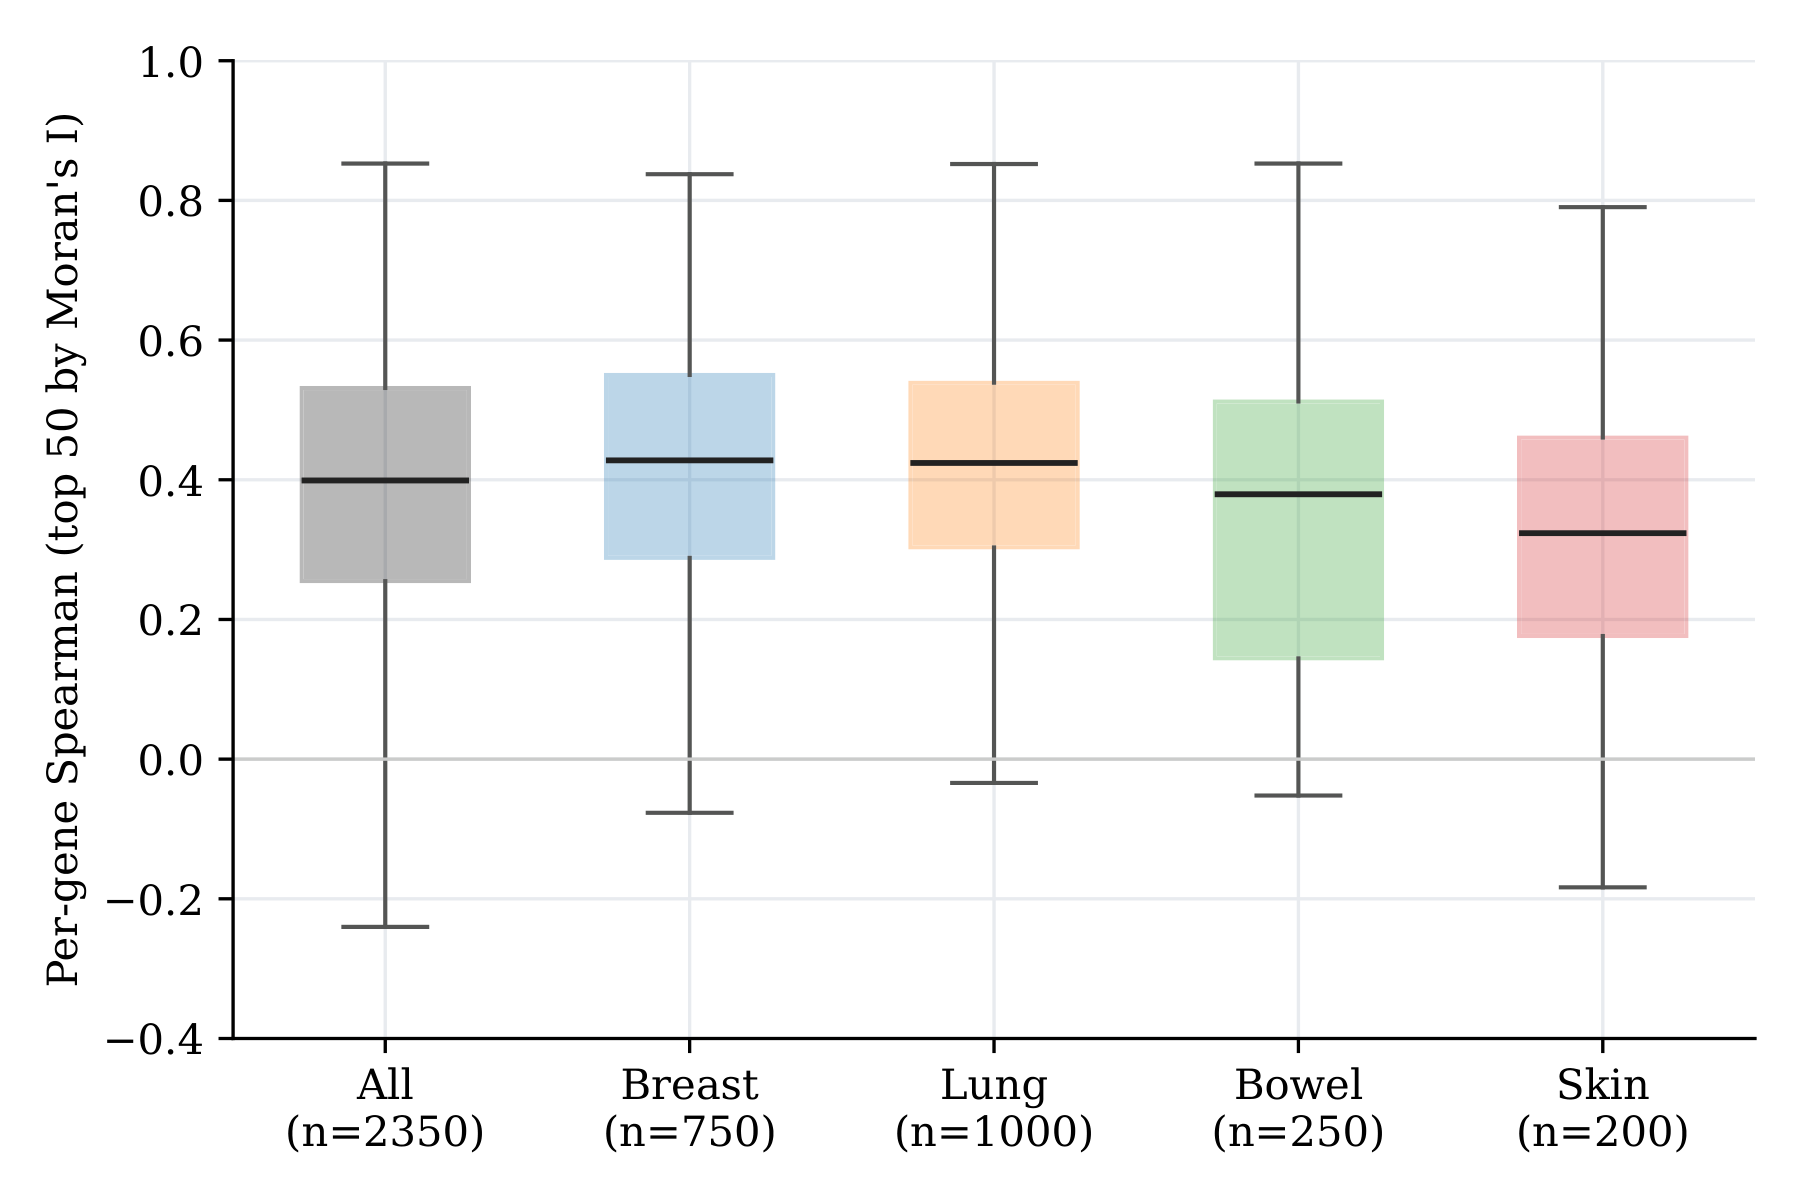
\includegraphics[width=\linewidth]{spearman_top50_box.png}
    \caption{Top 50 genes per slide.}
    \label{fig:spearman}
  \end{subfigure}
  \hfill
  \begin{subfigure}{0.48\linewidth}
    \centering
    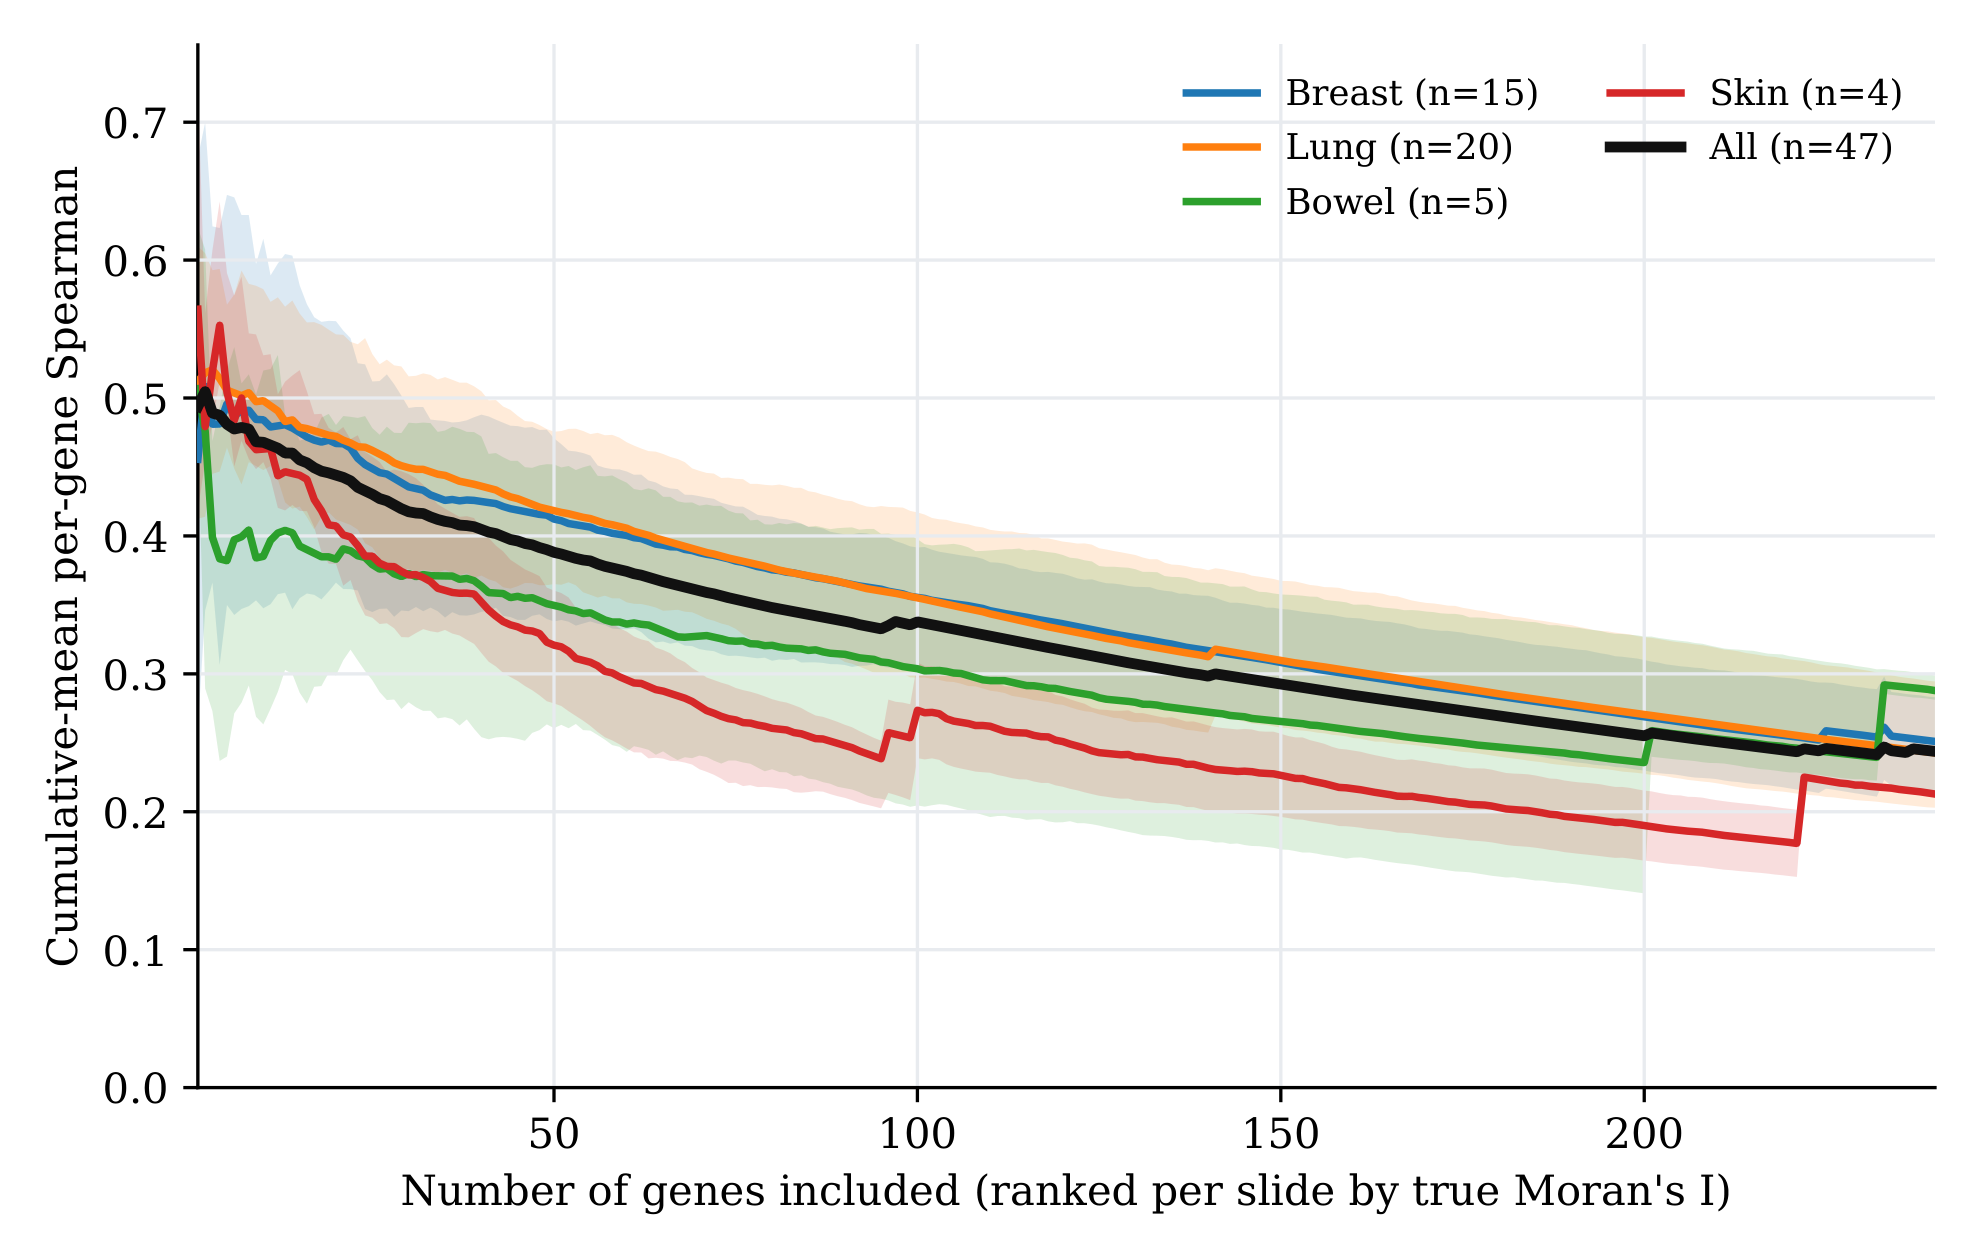
\includegraphics[width=\linewidth]{spearman_vs_ngenes.png}
    \caption{Full panel.}
    \label{fig:ngenes}
  \end{subfigure}
  \caption{Held-out HEST-1k recovery with inferred layouts. Every slide ranks its
  own genes by descending true Moran's I. (a) Distribution of per-gene Spearman
  over each slide's 50 highest-ranked genes, pooled across the group's slides, so
  one observation is one gene on one slide and every slide contributes 50 values;
  boxes give the interquartile range and whiskers the full extent. (b) The same
  quantity read cumulatively: each line is the mean across slides of the running
  average over the first $n$ genes, with shaded bands the interquartile range
  across slides at that gene count. Skin ($n=4$) and bowel ($n=5$) contribute too
  few slides for their bands to be read as distribution estimates. Slides also
  carry different panel sizes, so each average in (b) is taken over the slides
  that still have genes remaining: all 47 contribute through 50 genes, 44 by 100,
  and 35 by 240, which is what produces the steps in the right-hand tail.}
  \label{fig:heldout}
\end{figure}

Aggregate correlations do not show what the predictions look like in tissue. We
therefore examine one biologically informative gene from each tissue, always
showing measured expression beside Astra's prediction.

\smallskip
\begin{figure}[!htbp]
  \centering
  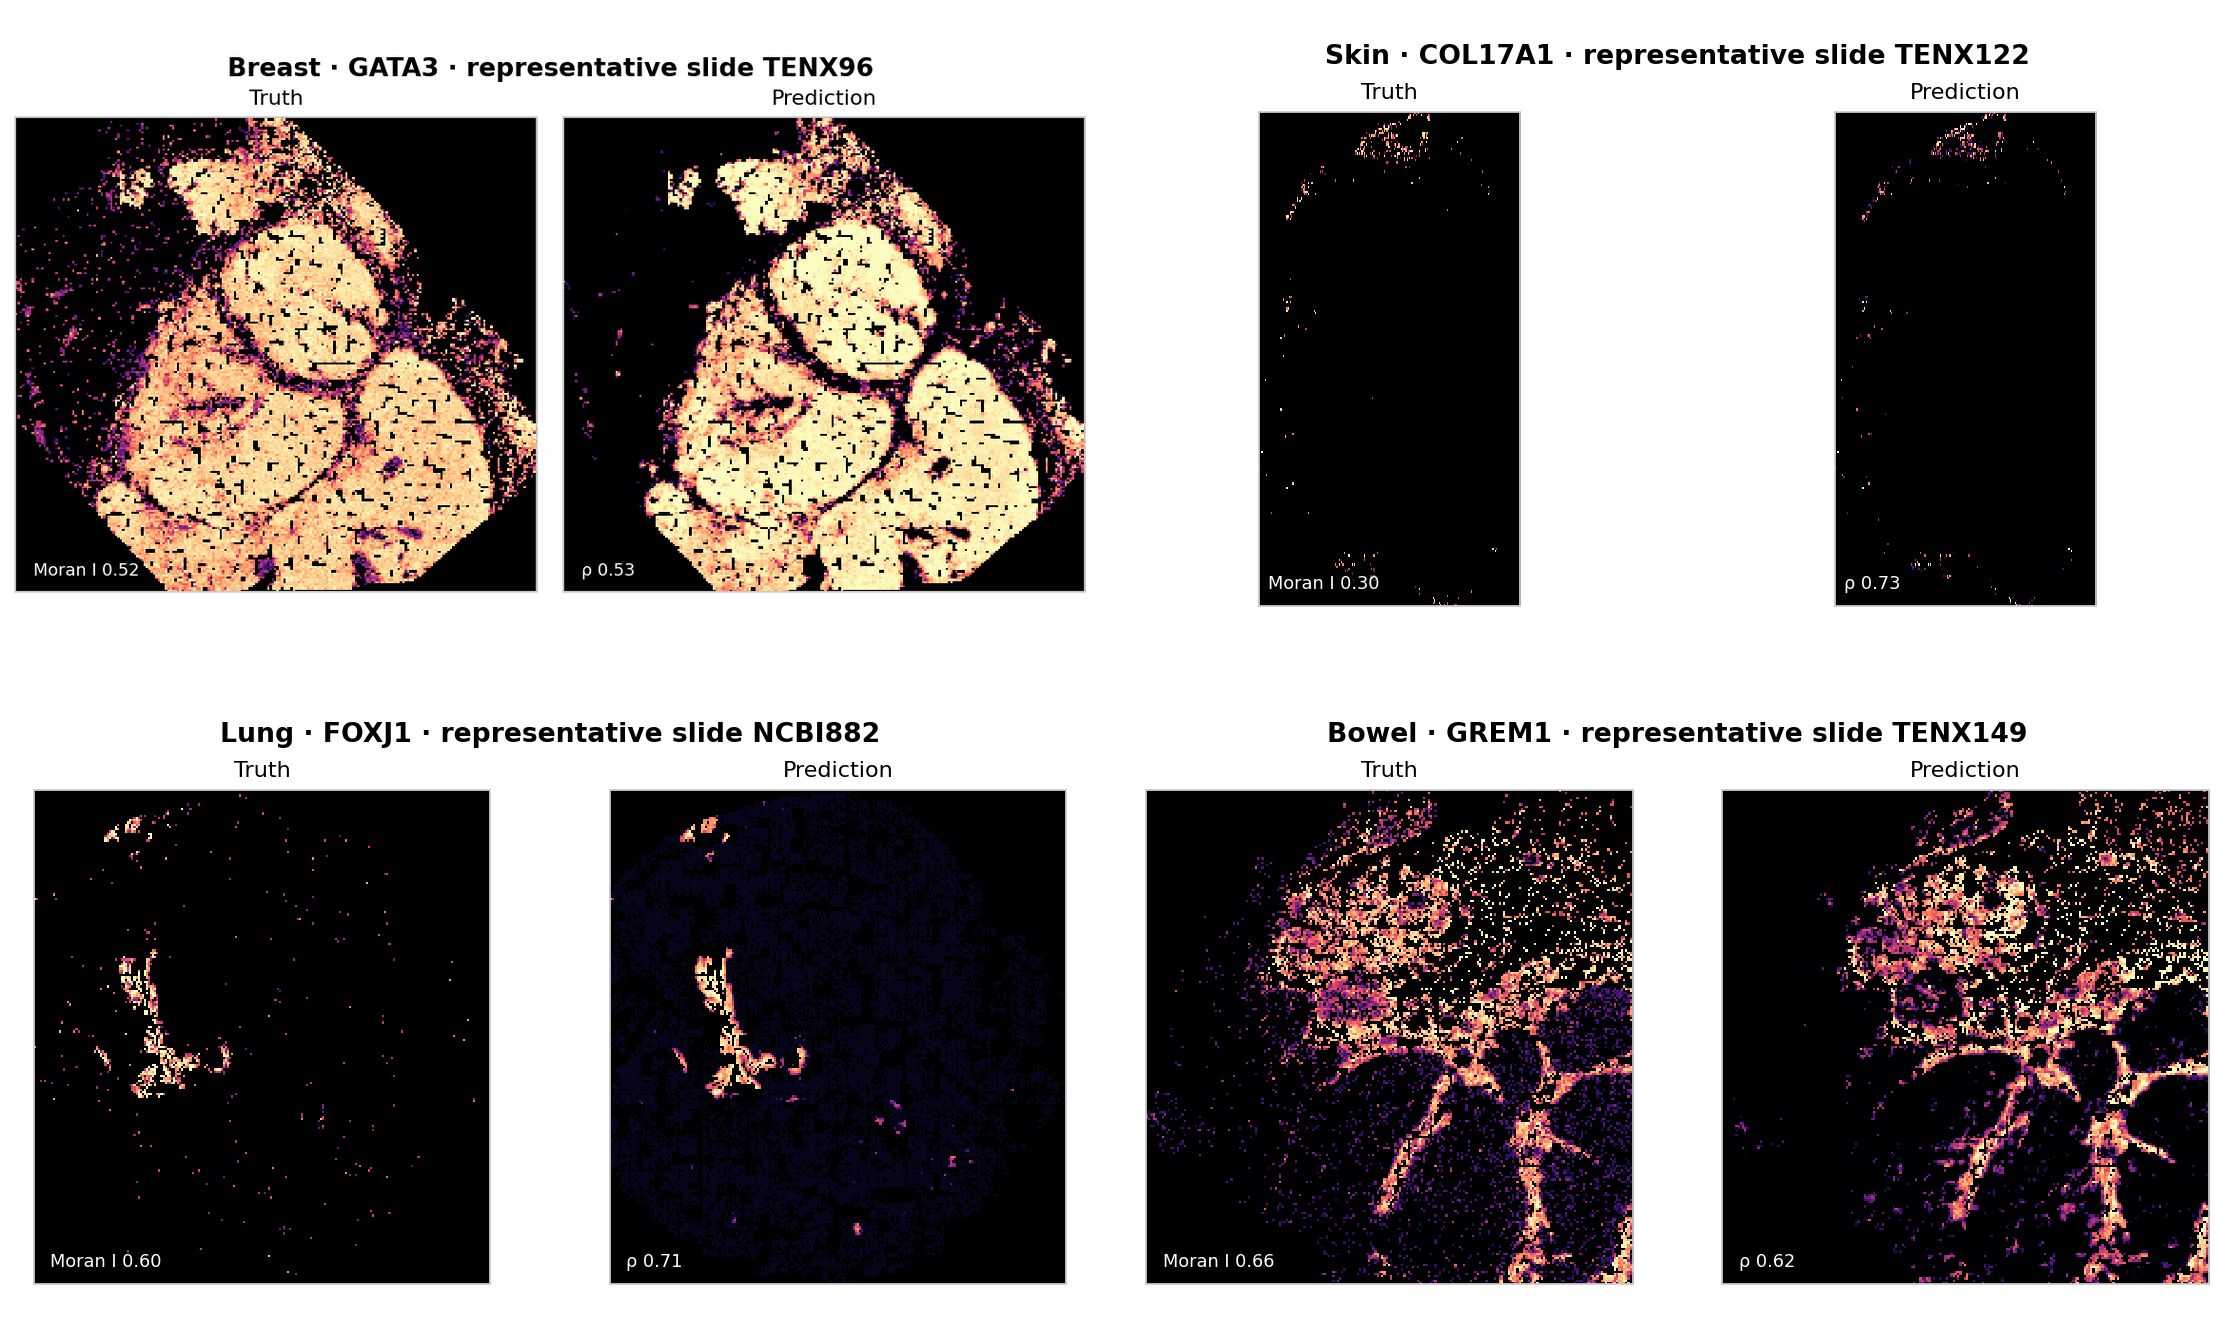
\includegraphics[width=0.96\linewidth]{marker_panel.png}
  \caption{Measured (left within each panel) and Astra-predicted
  (right) expression for GATA3 in breast, COL17A1 in skin, FOXJ1 in lung, and
  GREM1 in bowel.}
  \label{fig:marker_panel}
\end{figure}

These maps test whether Astra places high-expression domains and compartment
boundaries correctly rather than only matching a slide-level distribution,
spanning four distinct morphology--expression relationships. GATA3 marks luminal
mammary epithelium and estrogen-receptor signaling, a defining regulator of
luminal breast-cancer identity~\cite{gata3_breast}; COL17A1 anchors basal
keratinocytes through hemidesmosomes and marks a distinct basal skin
compartment~\cite{col17_skin}; FOXJ1 drives motile-cilia differentiation,
localizing ciliated airway epithelium against surrounding lung~\cite{foxj1_lung};
and GREM1, a BMP antagonist, marks a cancer-promoting stromal program in
colorectal tissue~\cite{grem1_crc}. Astra recovers these domains with Spearman
correlations of 0.53, 0.73, 0.71, and 0.62, respectively. These are qualitative
spatial sanity checks chosen to cover distinct compartments (a nuclear luminal
regulator, a basal adhesion protein, a ciliogenesis factor, and a secreted
stromal antagonist), not the highest-correlation genes or evidence that they are
privileged biomarkers; the held-out aggregate analyses
(Figure~\ref{fig:heldout}) provide the quantitative assessment.

\subsection{Astra recovers pathologist-annotated cell composition}
\label{sec:panoptils}

The evaluations above compare Astra against measured transcripts. A different
and stricter question is whether the predicted transcriptome encodes what a
pathologist actually reads off the slide: how much of a field is tumor, immune
infiltrate, and stroma. That composition is not an arbitrary target:
tumor-infiltrating lymphocyte density is prognostic across breast-cancer
subtypes~\cite{tils_denkert} and has a standardized scoring protocol precisely
because visual estimation is subjective~\cite{tils_working_group}. Recovering it
from H\&E-derived expression therefore tests biological fidelity against a
readout with established clinical meaning. We use
PanopTILs~\cite{panoptils}, which fuses the BCSS region annotations~\cite{bcss}
with nucleus-level classifications into 1{,}317 exhaustively annotated
$1024\times1024$ regions of interest at $0.25\,\mu$m/pixel drawn from 118 TCGA
breast-cancer slides. Every nucleus in the annotated field carries a manual class
label, which gives each ROI a ground-truth fraction of tumor/epithelial,
lymphocytic, and stromal cells. Nothing here is in distribution for Astra: the
image-to-expression model is trained only on HEST-1k Xenium slides, sees no TCGA
image, and is never shown a cell-type label.

Astra stays frozen. For each ROI we take the central $512\times512$-pixel crop,
which at $0.25\,\mu$m/pixel is exactly the $128\,\mu$m field in which PanopTILs
concentrates its manual nucleus annotations, resample it to the model's working
resolution, and run the density and expression heads to decode cells and predict
their expression. Averaging the decoded cells (median 155 per ROI) gives one
1{,}656-gene profile per ROI. A three-output multilayer perceptron then maps that
profile to the three fractions (Methods~\ref{met:panoptils}), trained in the
patient-grouped five-fold split released with
Path2Space~\cite{path2space} so that no slide is split across folds, with genes
and hyperparameters selected only inside each training fold. Following the same
protocol, we score per-slide Pearson correlation between predicted and manual
fractions and presence/absence AUROC, averaged over the 20 slides carrying at
least 20 ROIs.

\begin{figure}[!htbp]
  \centering
  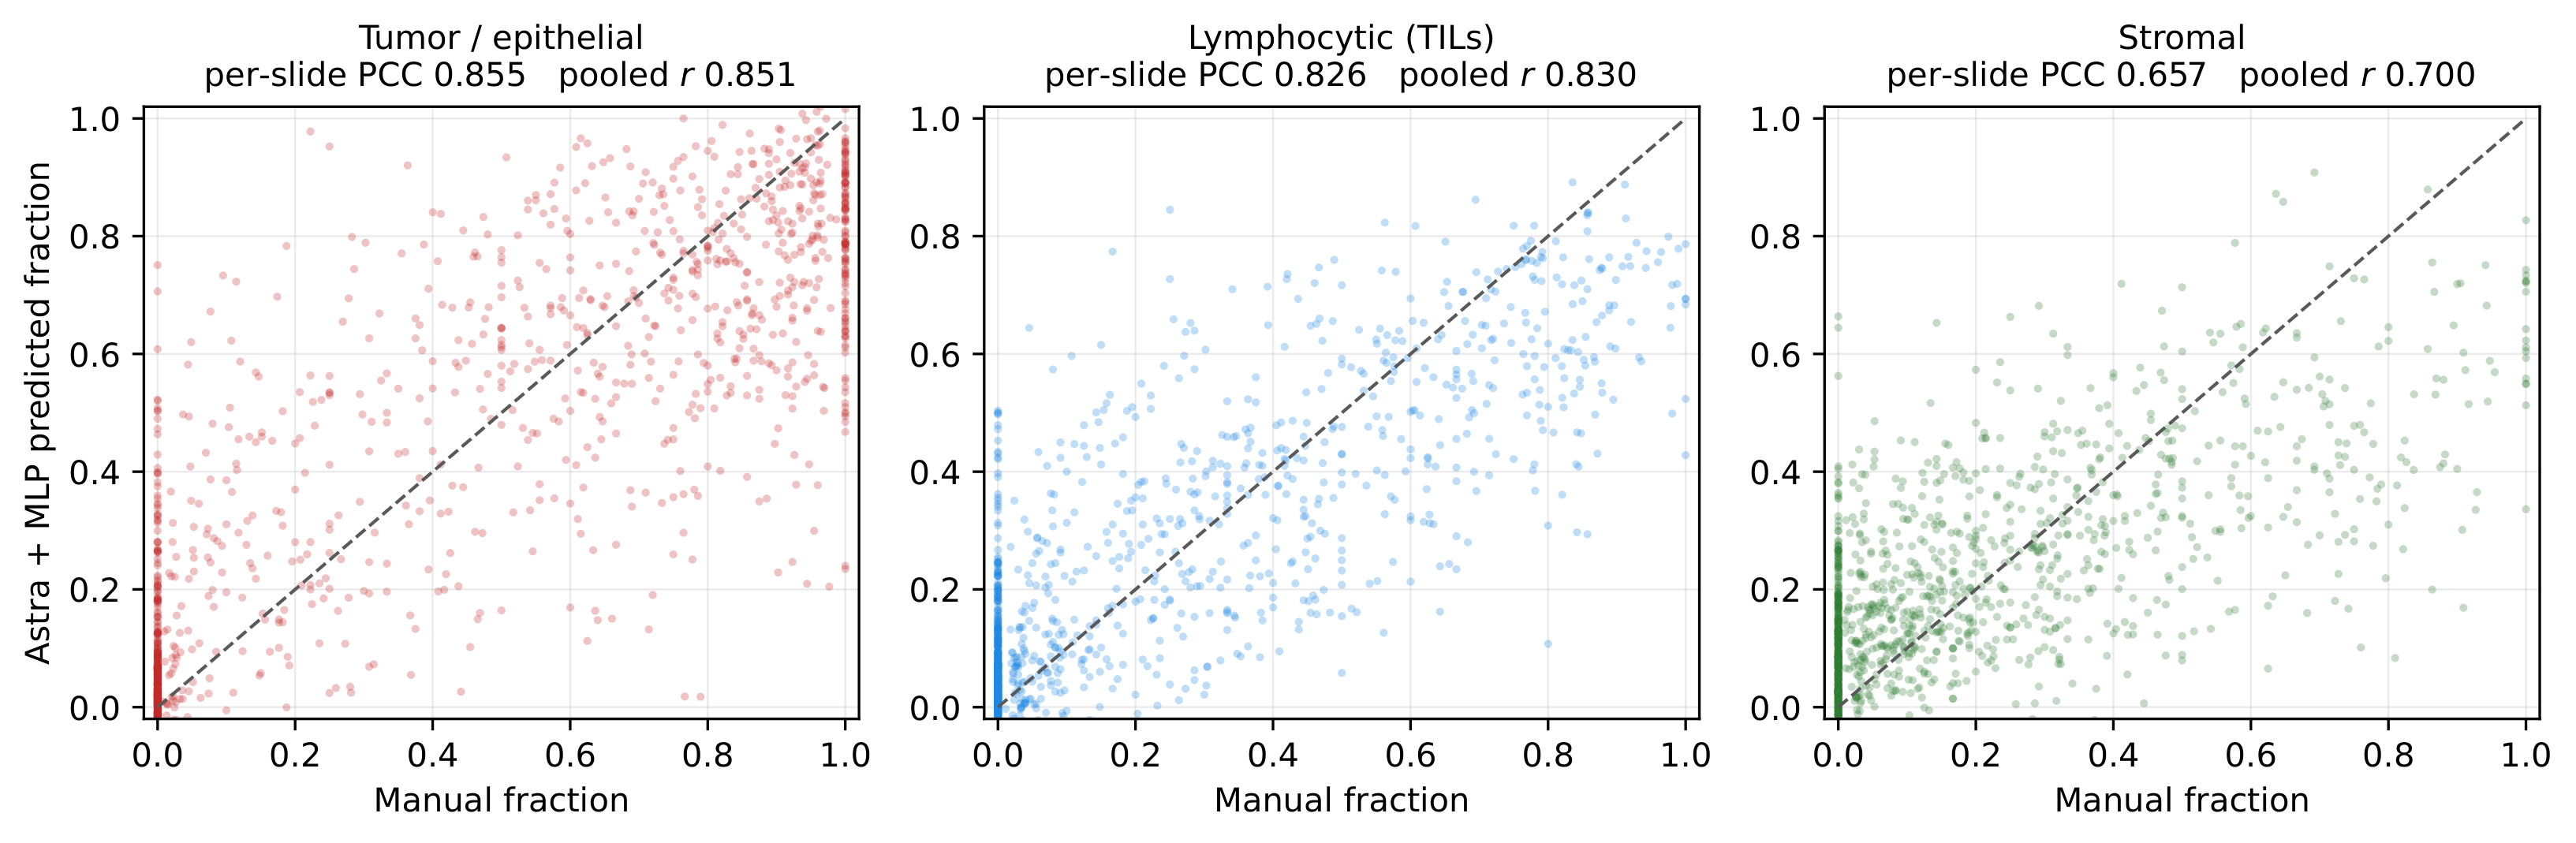
\includegraphics[width=0.98\linewidth]{panoptils_scatter.png}
  \caption{Held-out predicted versus manually annotated cell fractions
  across all 1{,}317 PanopTILs ROIs, with the identity line dashed. Panel titles
  give the per-slide correlation averaged over the 20 qualifying slides and the
  correlation pooled over all ROIs.}
  \label{fig:panoptils_scatter}
\end{figure}

Predicted fractions track the manual counts closely for tumor and lymphocytes:
per-slide PCC is 0.855 for tumor/epithelial and
0.826 for lymphocytic nuclei, with pooled correlations of 0.851 and 0.830 over all
1{,}317 ROIs (Figure~\ref{fig:panoptils_scatter}). Stroma is harder (per-slide
PCC 0.657, pooled 0.700) and far more variable between slides, ranging from 0.08
to 0.92, which is consistent with fibroblasts being the class whose morphology
and expression overlap most with the surrounding tissue. Treated as a
presence/absence call rather than a magnitude, the same predictions reach a mean
per-slide AUROC of 0.915, 0.873, and 0.839 for tumor, lymphocytic, and stromal
cells (Figure~\ref{fig:panoptils_roc}), so the model reliably answers whether a
compartment is present in a field even where it misestimates how much of it there
is.

\begin{figure}[!htbp]
  \centering
  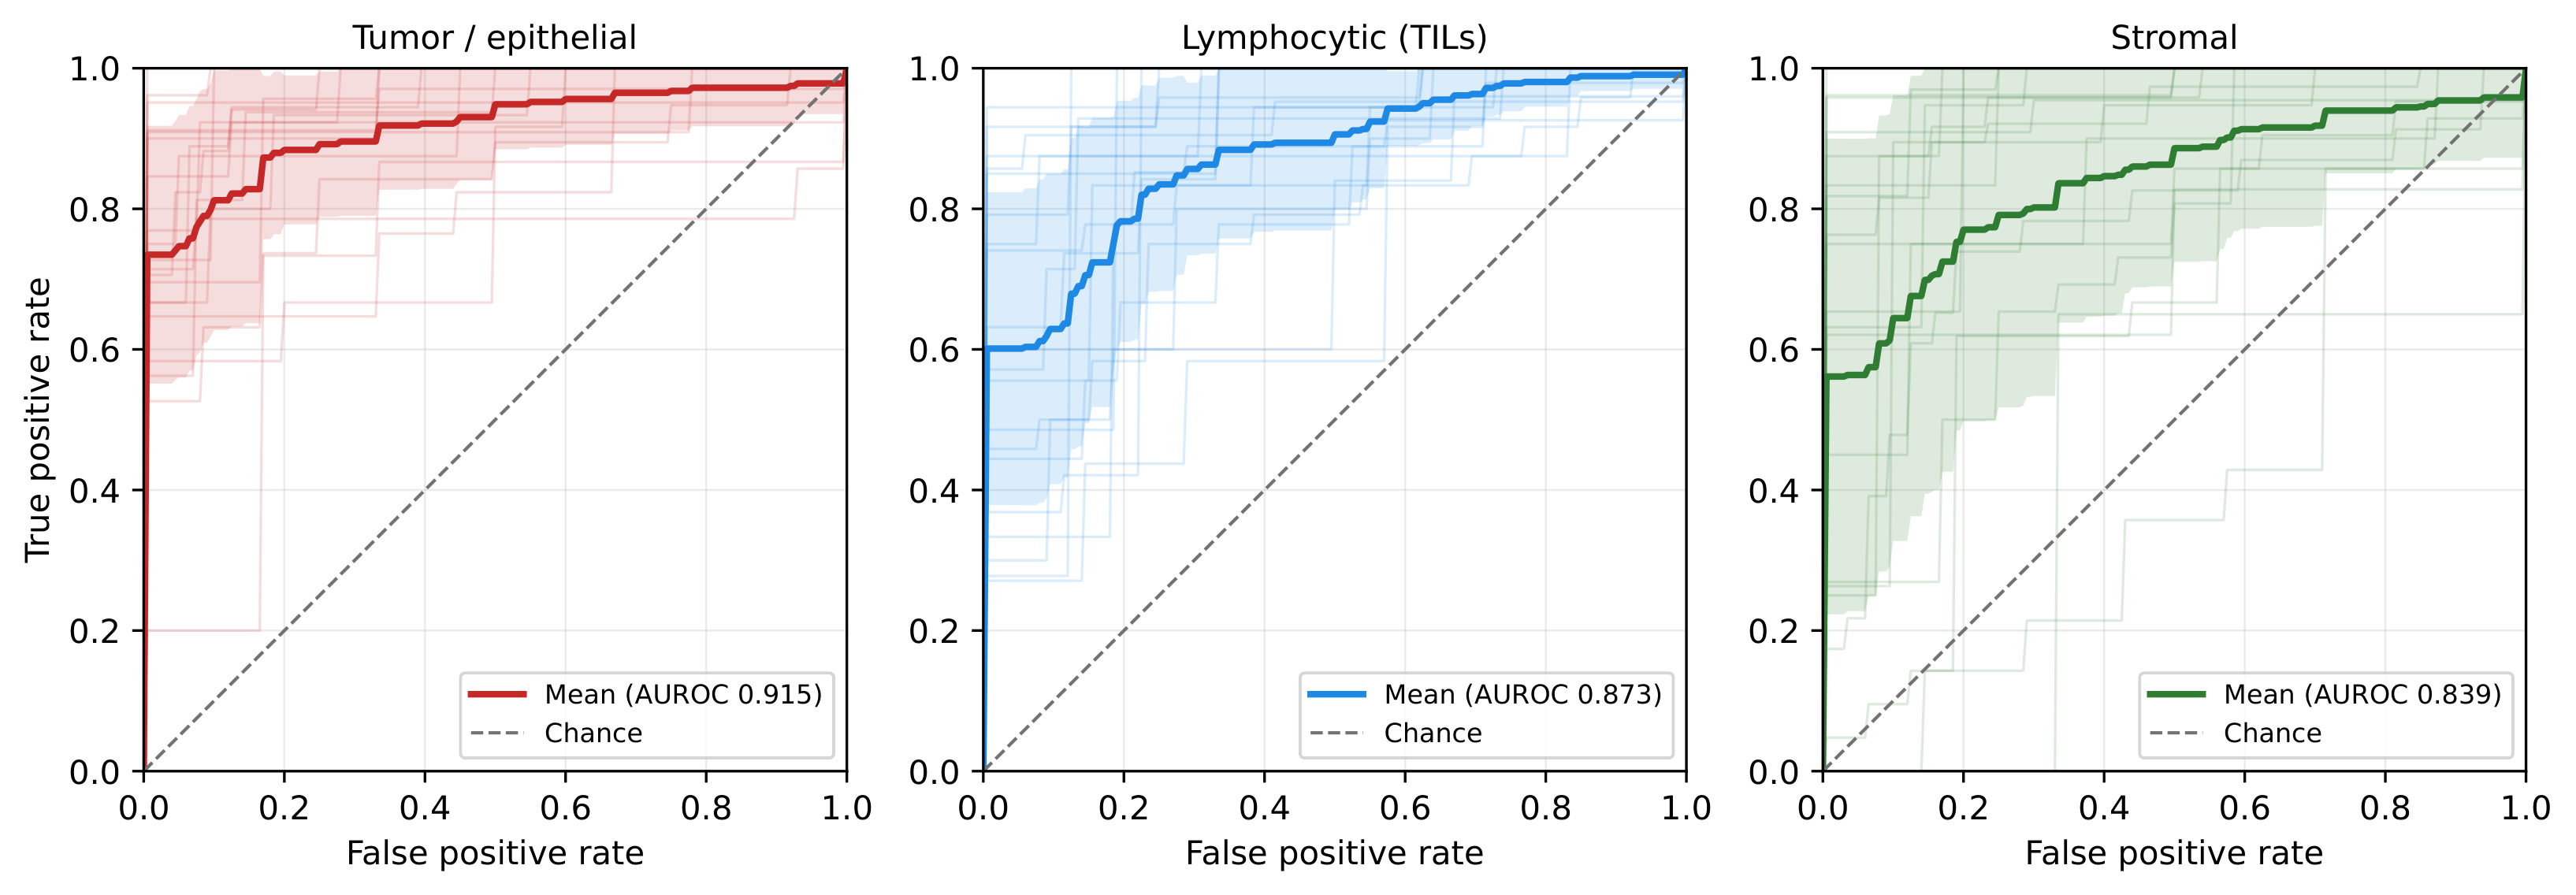
\includegraphics[width=0.98\linewidth]{panoptils_roc.png}
  \caption{Presence/absence ROC curves per cell type. Thin lines are the
  20 individual slides, the shaded band is $\pm1$ standard deviation, and the
  heavy line is the mean curve.}
  \label{fig:panoptils_roc}
\end{figure}

Because Path2Space reports this exact benchmark, the comparison isolates the
expression model. The ROIs, the fold assignment, the gene-selection rule, and the
regressor architecture and hyperparameters are all theirs; only the inferred
expression fed into the probe differs. On that substitution Astra improves every
one of the six reported scores (Figure~\ref{fig:panoptils_benchmark}): per-slide
PCC rises from 0.793 to 0.855 for tumor, 0.789 to 0.826 for lymphocytes, and
0.592 to 0.657 for stroma, and presence AUROC from 0.876 to 0.915, 0.858 to
0.873, and 0.836 to 0.839. The margin is widest on the magnitude metric and
narrowest on stromal detection, where both models are close to the same ceiling.
The comparison also runs against the grain of the training data: Path2Space is
trained on breast spatial transcriptomics, whereas Astra is trained across breast,
lung, bowel, and skin and reaches the TCGA breast cohort as an out-of-cohort
transfer.

\begin{figure}[!htbp]
  \captionsetup{skip=3pt}
  \centering
  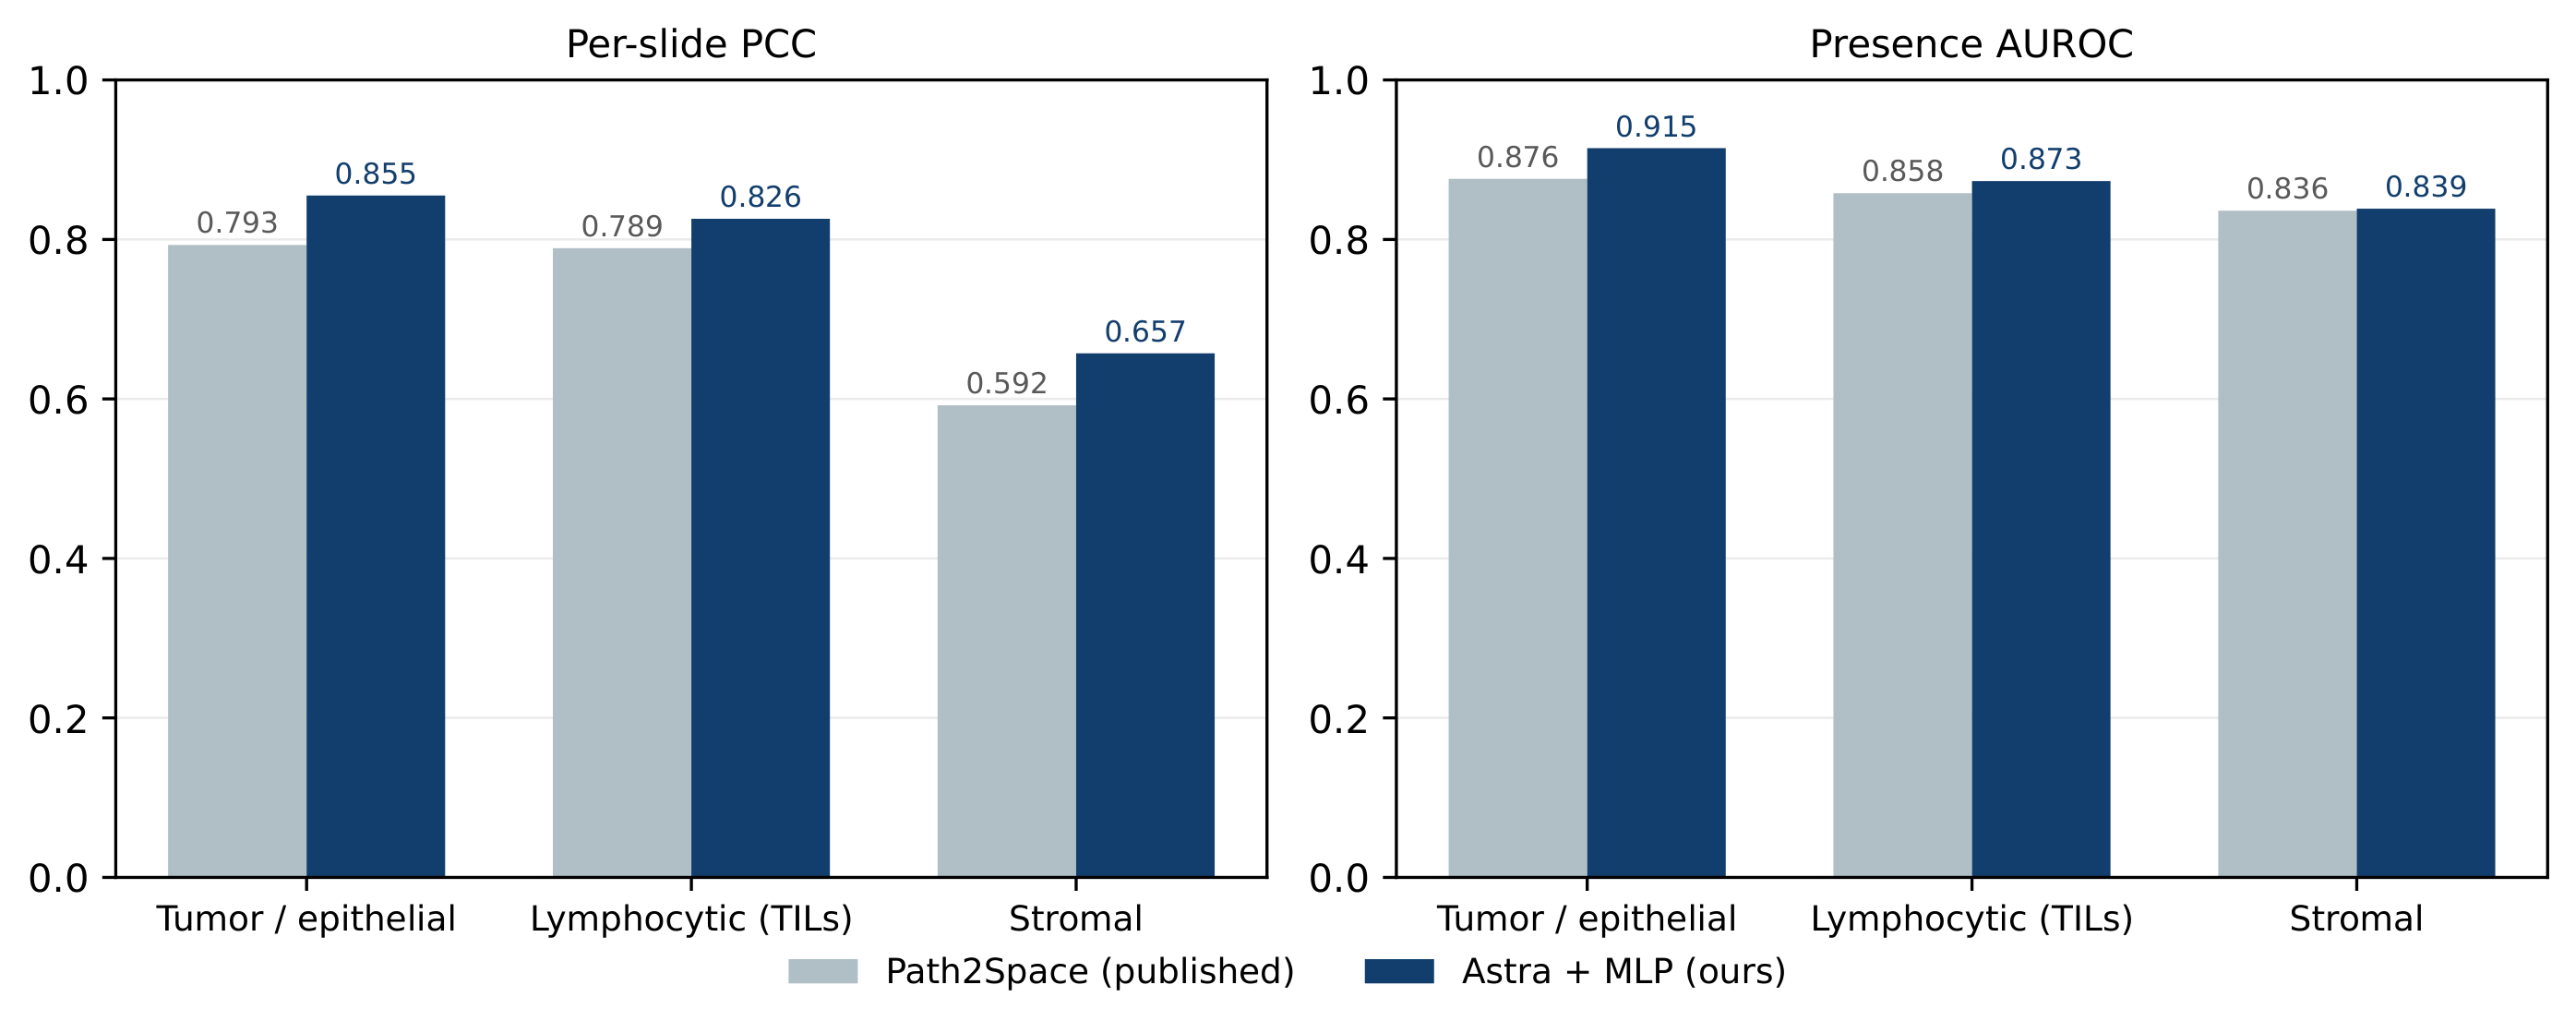
\includegraphics[width=0.90\linewidth]{panoptils_benchmark.png}
  \caption{Astra against the published Path2Space scores on the same
  1{,}317 ROIs, the same patient-grouped folds, and the same supervised probe.}
  \label{fig:panoptils_benchmark}
\end{figure}

Two limits frame this result. The probe is supervised, so it measures how much
cell-composition information the predicted transcriptome carries rather than
zero-shot deconvolution; we also applied reference-based
deconvolution~\cite{spacet} directly to the same profiles and it performed
substantially worse than the supervised probe, so we report the supervised route
throughout. And the labels are annotations of morphology, not an orthogonal
molecular assay, so agreement here establishes that Astra's expression is
consistent with expert reading of the tissue rather than independently validated
against measured cell types. With those caveats, a frozen cross-tissue expression
model recovers the compartment structure that TILs scoring depends on, on slides
and a cohort it never saw, and does so more accurately than a breast-specific
model built for the task.

\section{Architecture and data}
\label{sec:arch}

Astra uses a frozen H\&E image encoder to convert each tissue patch into visual
tokens, followed by a shared transformer trunk that integrates morphology across
the patch (Methods~\ref{met:arch}). From this representation the model branches into three heads
(Figure~\ref{fig:arch}): a per-cell expression head, a detector head that
predicts whether each target gene is non-zero in a given cell, and a density
head that predicts where cells lie within the patch.

\begin{figure}[!htbp]
  \centering
  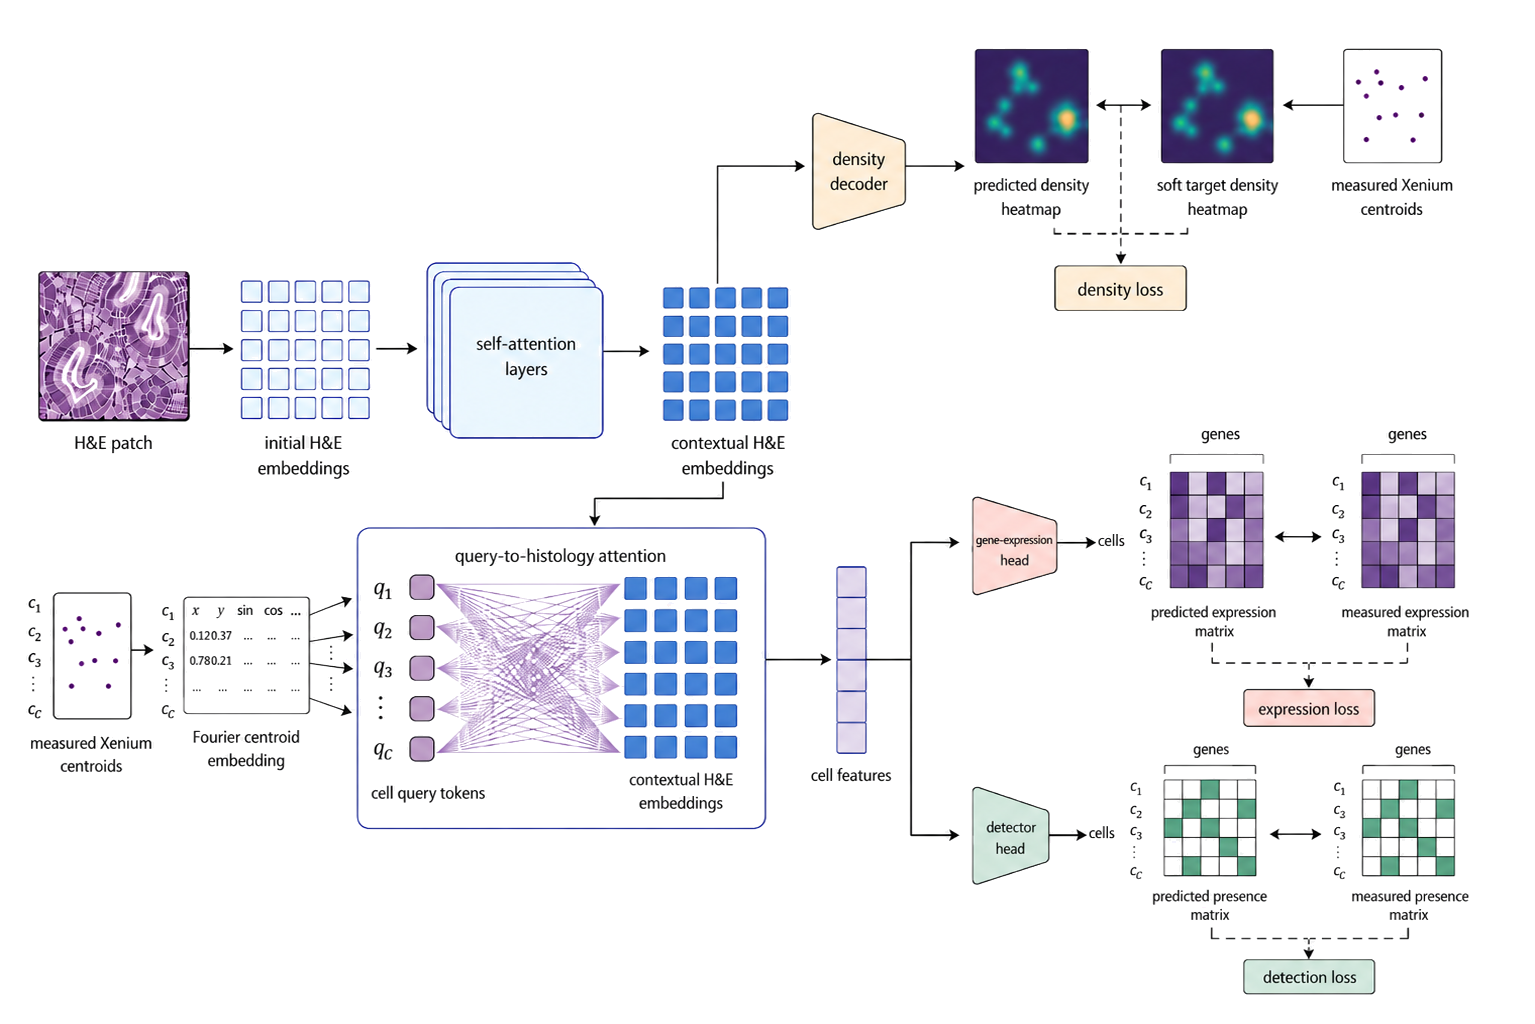
\includegraphics[width=0.88\linewidth]{model_arch.png}
  \caption{Astra's shared visual trunk and position-conditioned
  density, presence, and per-cell expression heads.}
  \label{fig:arch}
\end{figure}

The HEST-1k Xenium slides do not share a single gene panel: the breast, lung,
bowel, and skin assays each target a different set of transcripts. We reconcile
these per-tissue Xenium panels into one harmonized vocabulary and train Astra to
predict this fixed 1{,}656-gene output for every cell, regardless of which tissue
the patch comes from. This single output space is what the downstream clinical
analyses use: in Sections~\ref{sec:trastuzumab}--\ref{sec:msi} each patient is run
through the full 1{,}656-gene head, since those tasks operate per patient and never
require a common gene set across Xenium slides. The per-slide recovery in
Section~\ref{sec:recovery} reports on far fewer genes: each slide is scored on
its own top genes ranked by that slide's Moran's I, so the actual genes differ
from slide to slide. To average a top-$K$ statistic over all held-out slides on
equal footing, every slide must be able to supply $K$ genes, which caps $K$ at
the gene count of the smallest-panel slide, a few hundred genes. The number thus differs by application because of how
the metric is aggregated, not because the model emits a different panel.

The central design decision is that cells enter as queries defined by their own
centroids. Each cell's relative position inside the patch is encoded with a
Fourier embedding and used as a query that cross-attends to the patch's image
tokens, producing a feature for that specific cell. This avoids the object
mismatch of methods that detect nuclei on H\&E and then match them to a
transcriptomics segmentation: Astra has no matching step, because the centroids
themselves are the queries.

\begin{figure}[!htbp]
  \centering
  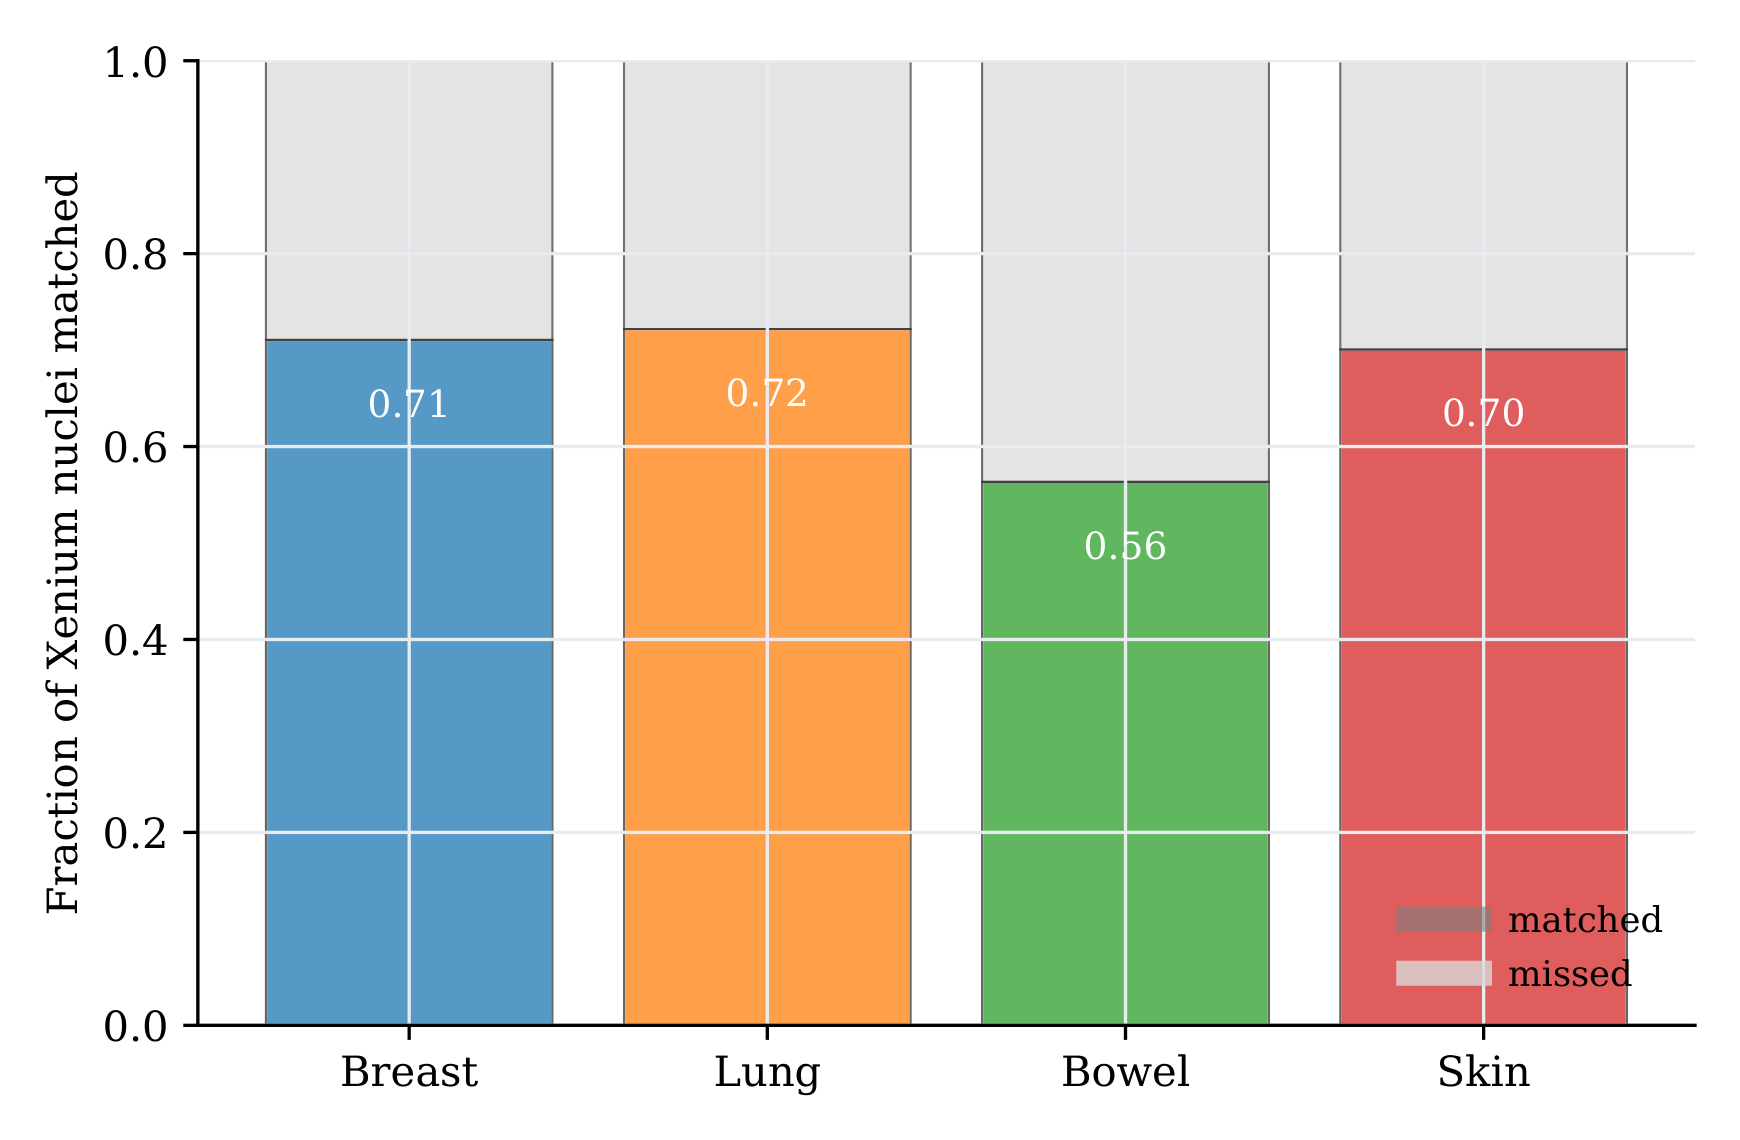
\includegraphics[width=0.46\linewidth]{detection_recall.png}
  \caption{Xenium nuclei matched to H\&E detections by tissue; grey,
  unmatched.}
  \label{fig:detection}
\end{figure}

This is a design decision about how training supervision is used, not a
benchmark against matching-based methods. H\&E detections and Xenium nuclei are
non-identical object sets: nearest-neighbor matching recovers 71\% of Xenium
cells in breast, 72\% in lung, 56\% in bowel, and 70\% in skin, leaving
28--44\% unmatched (Figure~\ref{fig:detection}). Matched-pair supervision must
therefore discard or misassign part of the measured transcriptome, whereas Astra
anchors training queries to measured Xenium centroids and uses every measured
cell, estimating their positions only at inference.

\begin{figure}[!htbp]
  \captionsetup{skip=3pt}
  \centering
  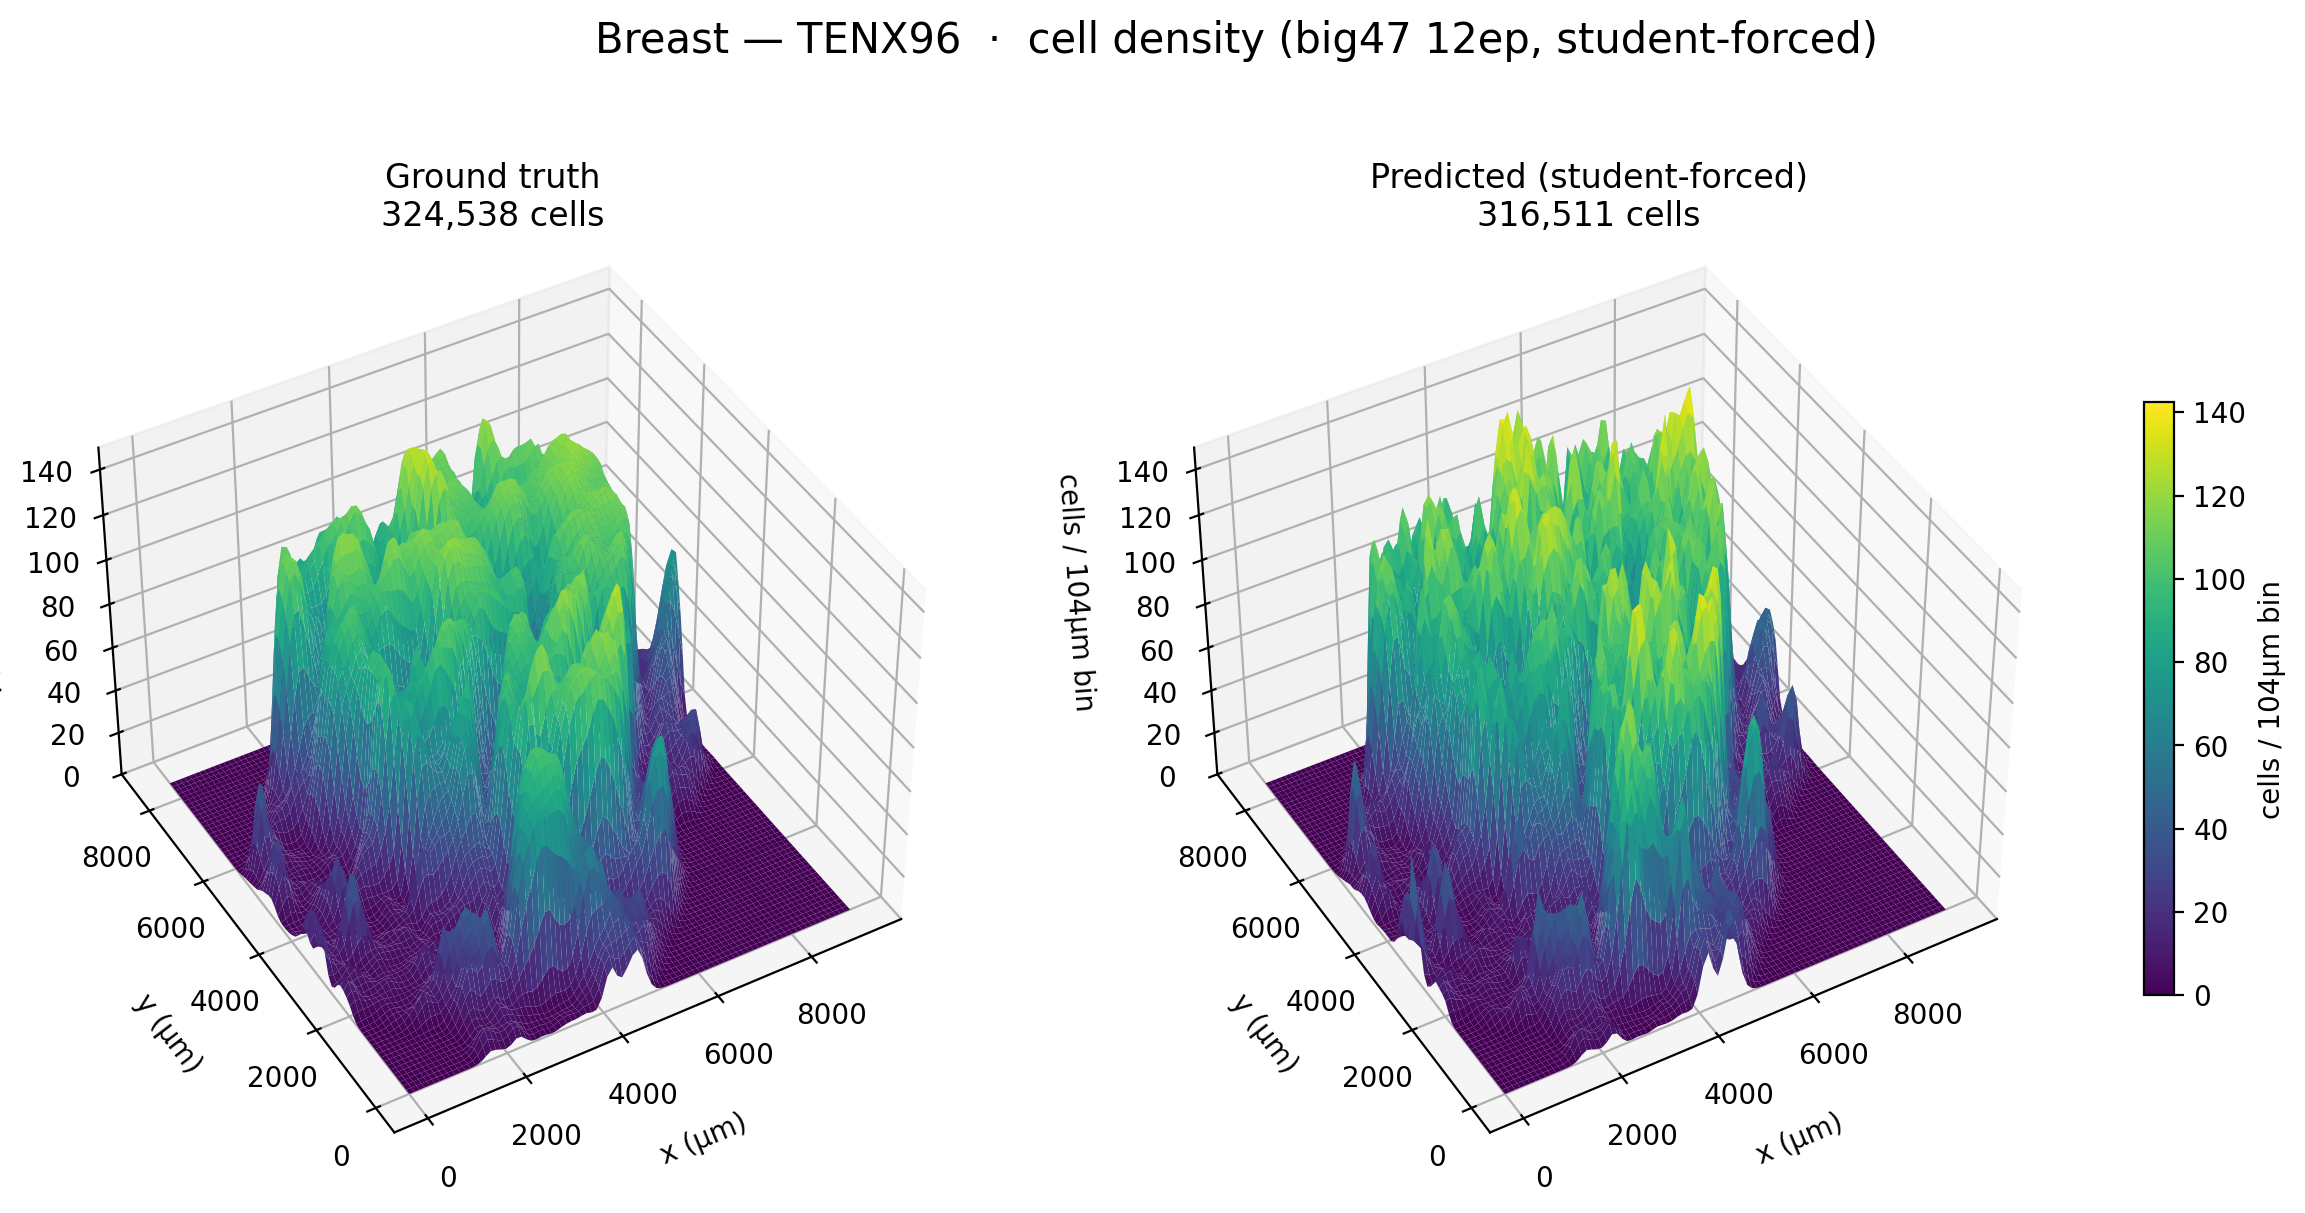
\includegraphics[width=0.62\linewidth]{density_surface.png}
  \caption{Measured and Astra-decoded density on held-out breast
  ($104\,\mu$m bins; 324{,}538 vs.\ 316{,}511 cells).}
  \label{fig:density}
\end{figure}

The density head is what makes inference H\&E-only. During training, cell queries
are placed at the true centroids while the density head learns the cellular
layout from a unit-mass Gaussian target (Methods~\ref{met:loss}); at inference Astra proposes that layout and queries expression at the
inferred positions. At inference the head emits a continuous density heatmap that
must be turned into discrete cell positions. We decode it adaptively
(Methods~\ref{met:decoding}): because the density target is built from unit-mass
Gaussians, integrating the map gives a cell count $C$, and comparing $C$ against
the number of resolvable local maxima says which decoder to trust. Where peaks
account for at least $80\%$ of $C$ we take those non-maximum-suppression peaks
directly; where the density saturates and peaks merge, so that fewer than $80\%$
of the predicted cells appear as distinct maxima, we instead place all $C$ cells
as density-weighted centroids by a Lloyd/centroidal-Voronoi relaxation, which
recovers the correct cell count in crowded regions where peak picking would
undercount. The decoded layout closely tracks the measured one both in total count
and in spatial distribution (Figure~\ref{fig:density}).

Because the decoded and measured cells are two independent point sets, we pair
them for scoring by greedy nearest-neighbor matching (Methods~\ref{met:recovery}): processed in increasing
distance, each measured cell claims its closest unclaimed predicted cell within a
distance gate set by the slide's typical cell spacing, giving one-to-one pairs
(unmatched cells count as misses or false positives), and per-gene Spearman
correlations are computed over these matched pairs. All recovery results in this
paper are scored in this fully H\&E-only setting, using Astra's decoded layout
rather than measured centroids.

The detector head addresses a different failure mode. A continuous head
trained with mean-squared error on $\log(1+x)$ never outputs hard zeros, so
absent genes emerge as small non-zero values and can fabricate infiltration
for markers such as PTPRC~\cite{cd45}. A separate head predicts whether each gene is
non-zero, and gating by that probability restores true absences. One fixed
threshold, selected on held-out validation slides, is used throughout. The
detector reaches AUROC 0.97 in lung, 0.94 in breast, 0.83 in bowel, and 0.80
in skin (pooled 0.94; Figure~\ref{fig:detroc}).

\begin{figure}[!htbp]
  \captionsetup{skip=3pt}
  \centering
  
\includegraphics[width=0.62\linewidth]{detector_roc.png}
  \caption{Held-out gene-presence detector ROC by tissue.}
  \label{fig:detroc}
\end{figure}

To sanity-check the training mixture and decide which tissues to keep, we trace
each held-out query patch back to the training patches that most helped or hurt
its prediction with influence functions. For a query patch $q$ and a training
candidate $c$ the FastInf score is
$I(c,q)=-(\nabla_\theta L_c)^{\top}\hat{G}_\lambda^{-1}(\nabla_\theta \ell_q)$,
where $\ell_q$ is the all-genes MSE loss on the held-out patch and $L_c$ the same
loss on the candidate. The curvature term $\hat{G}_\lambda$ is a block-diagonal
generalized Fisher matrix accumulated over a Fisher subsample of $N_F=1{,}024$
training patches ($64$ batches of $16$) as
$\hat G\approx\frac{1}{N_F}\sum_i g_ig_i^{\top}$ per trainable matrix block (a
diagonal Fisher for vector blocks), then \emph{damped} by adding a multiple of
the identity before inversion,
\[
\hat G_\lambda=\hat G+\lambda I ,
\]
and inverted with a Schulz hyperpower iteration (HyperINF). The damping term
$\lambda$ is what makes the inverse well-conditioned: the empirical Fisher is
low-rank and near-singular at this subsample size, so $\lambda$ floors its
spectrum and bounds $\lVert\hat G_\lambda^{-1}\rVert$, trading curvature fidelity
for numerical stability. We use $\lambda=0.01$, the smallest value in a
$\lambda\in\{0.01,0.05,0.1\}$ sweep that still inverts stably, since larger
damping drives $\hat G_\lambda^{-1}\!\to\!\lambda^{-1}I$ and degrades the score
toward a plain gradient dot product. The score is signed: a negative value marks
a beneficial (proponent) patch that lowers the query's loss, a positive value a
harmful (opponent) one. Scoring each query against the whole training set is
intractable, so we narrow candidates in two stages. First a FastIF-style
retrieval step picks \emph{which} patches are eligible: for each query we take
its $k=10{,}000$ nearest training patches by L2 distance between frozen Gigapath
class-token features, a purely visual-similarity filter. We then compute the
influence score above for that shortlist and rank patches by the score itself, so
``most influential'' is decided by influence, not by feature distance. We report
raw (non-cosine) scores at $\lambda=0.01$ and $k=10{,}000$ over $1{,}024$
held-out queries.

The recovered relationships pass an obvious sanity check and surface a useful
data decision. Beneficial influence is overwhelmingly same-tissue and
morphologically matched: a query's strongest proponents are training patches of
the same tissue that share its morphology (same-tissue fraction 0.96 lung, 0.92
breast, 0.86 pancreas, 0.84 skin; Figure~\ref{fig:influence_heatmap}). The
systematic exception is bowel, whose beneficial influencers are only 0.58 bowel
and draw heavily on pale fibrous/stromal patches from pancreas (0.26) and breast
(0.08), so influence tracks shared morphology, not the tissue label. That is what
tells us to include the pancreas slides even though Astra is not intended for
pancreas inference: pancreas is the single largest cross-tissue source of
beneficial signal for bowel, a tissue we do report on. The qualitative panel
shows the same pattern patch by patch, with each query retrieving same-tissue
twins as its top proponents while bowel pulls in breast and pancreas stroma
(Figure~\ref{fig:influence_qual}).

\begin{figure}[!htbp]
  \centering
  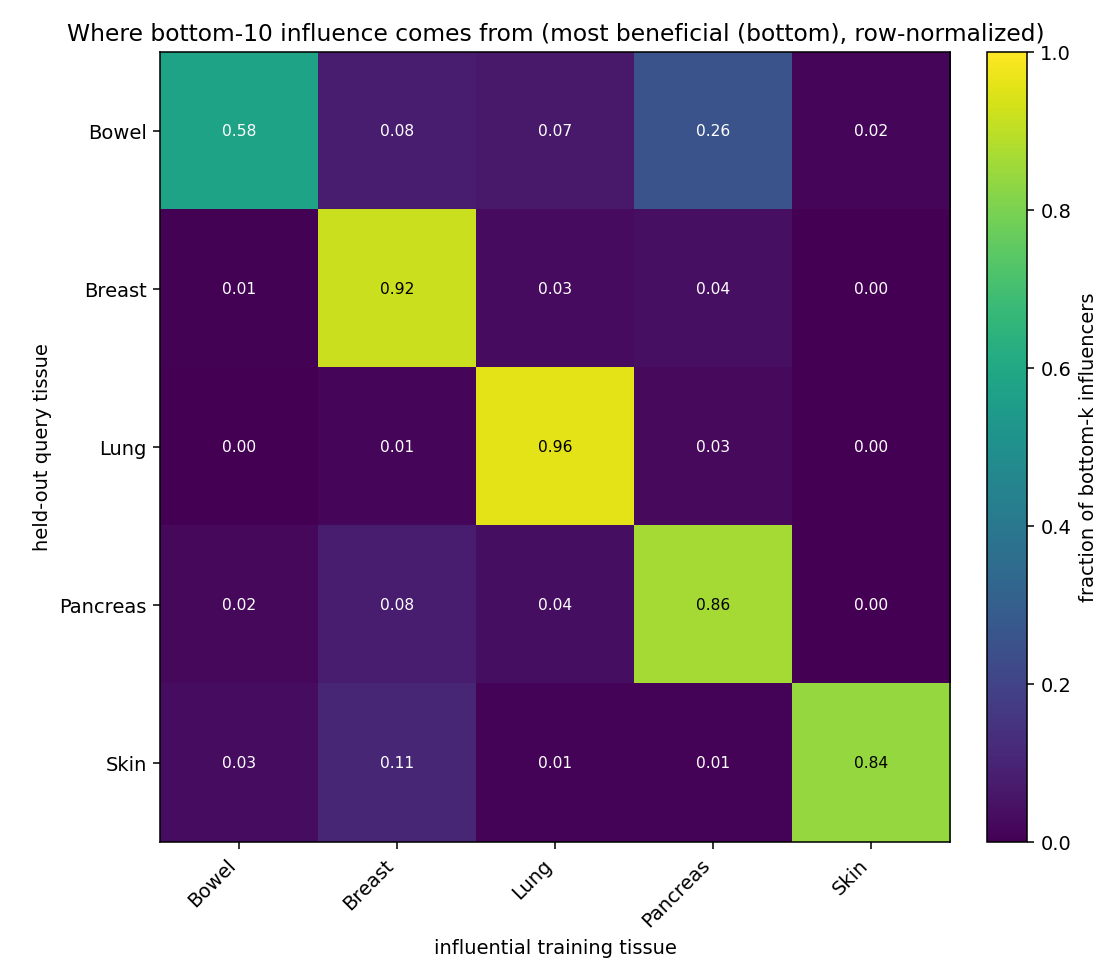
\includegraphics[width=0.8\linewidth]{influence_tissue_heatmap.png}
  \caption{Where beneficial (bottom-10) influence comes from, row-normalized by
  held-out query tissue. Proponents are dominated by the same tissue, with bowel
  the exception (strong pancreas contribution).}
  \label{fig:influence_heatmap}
\end{figure}

\begin{figure}[!htbp]
  \centering
  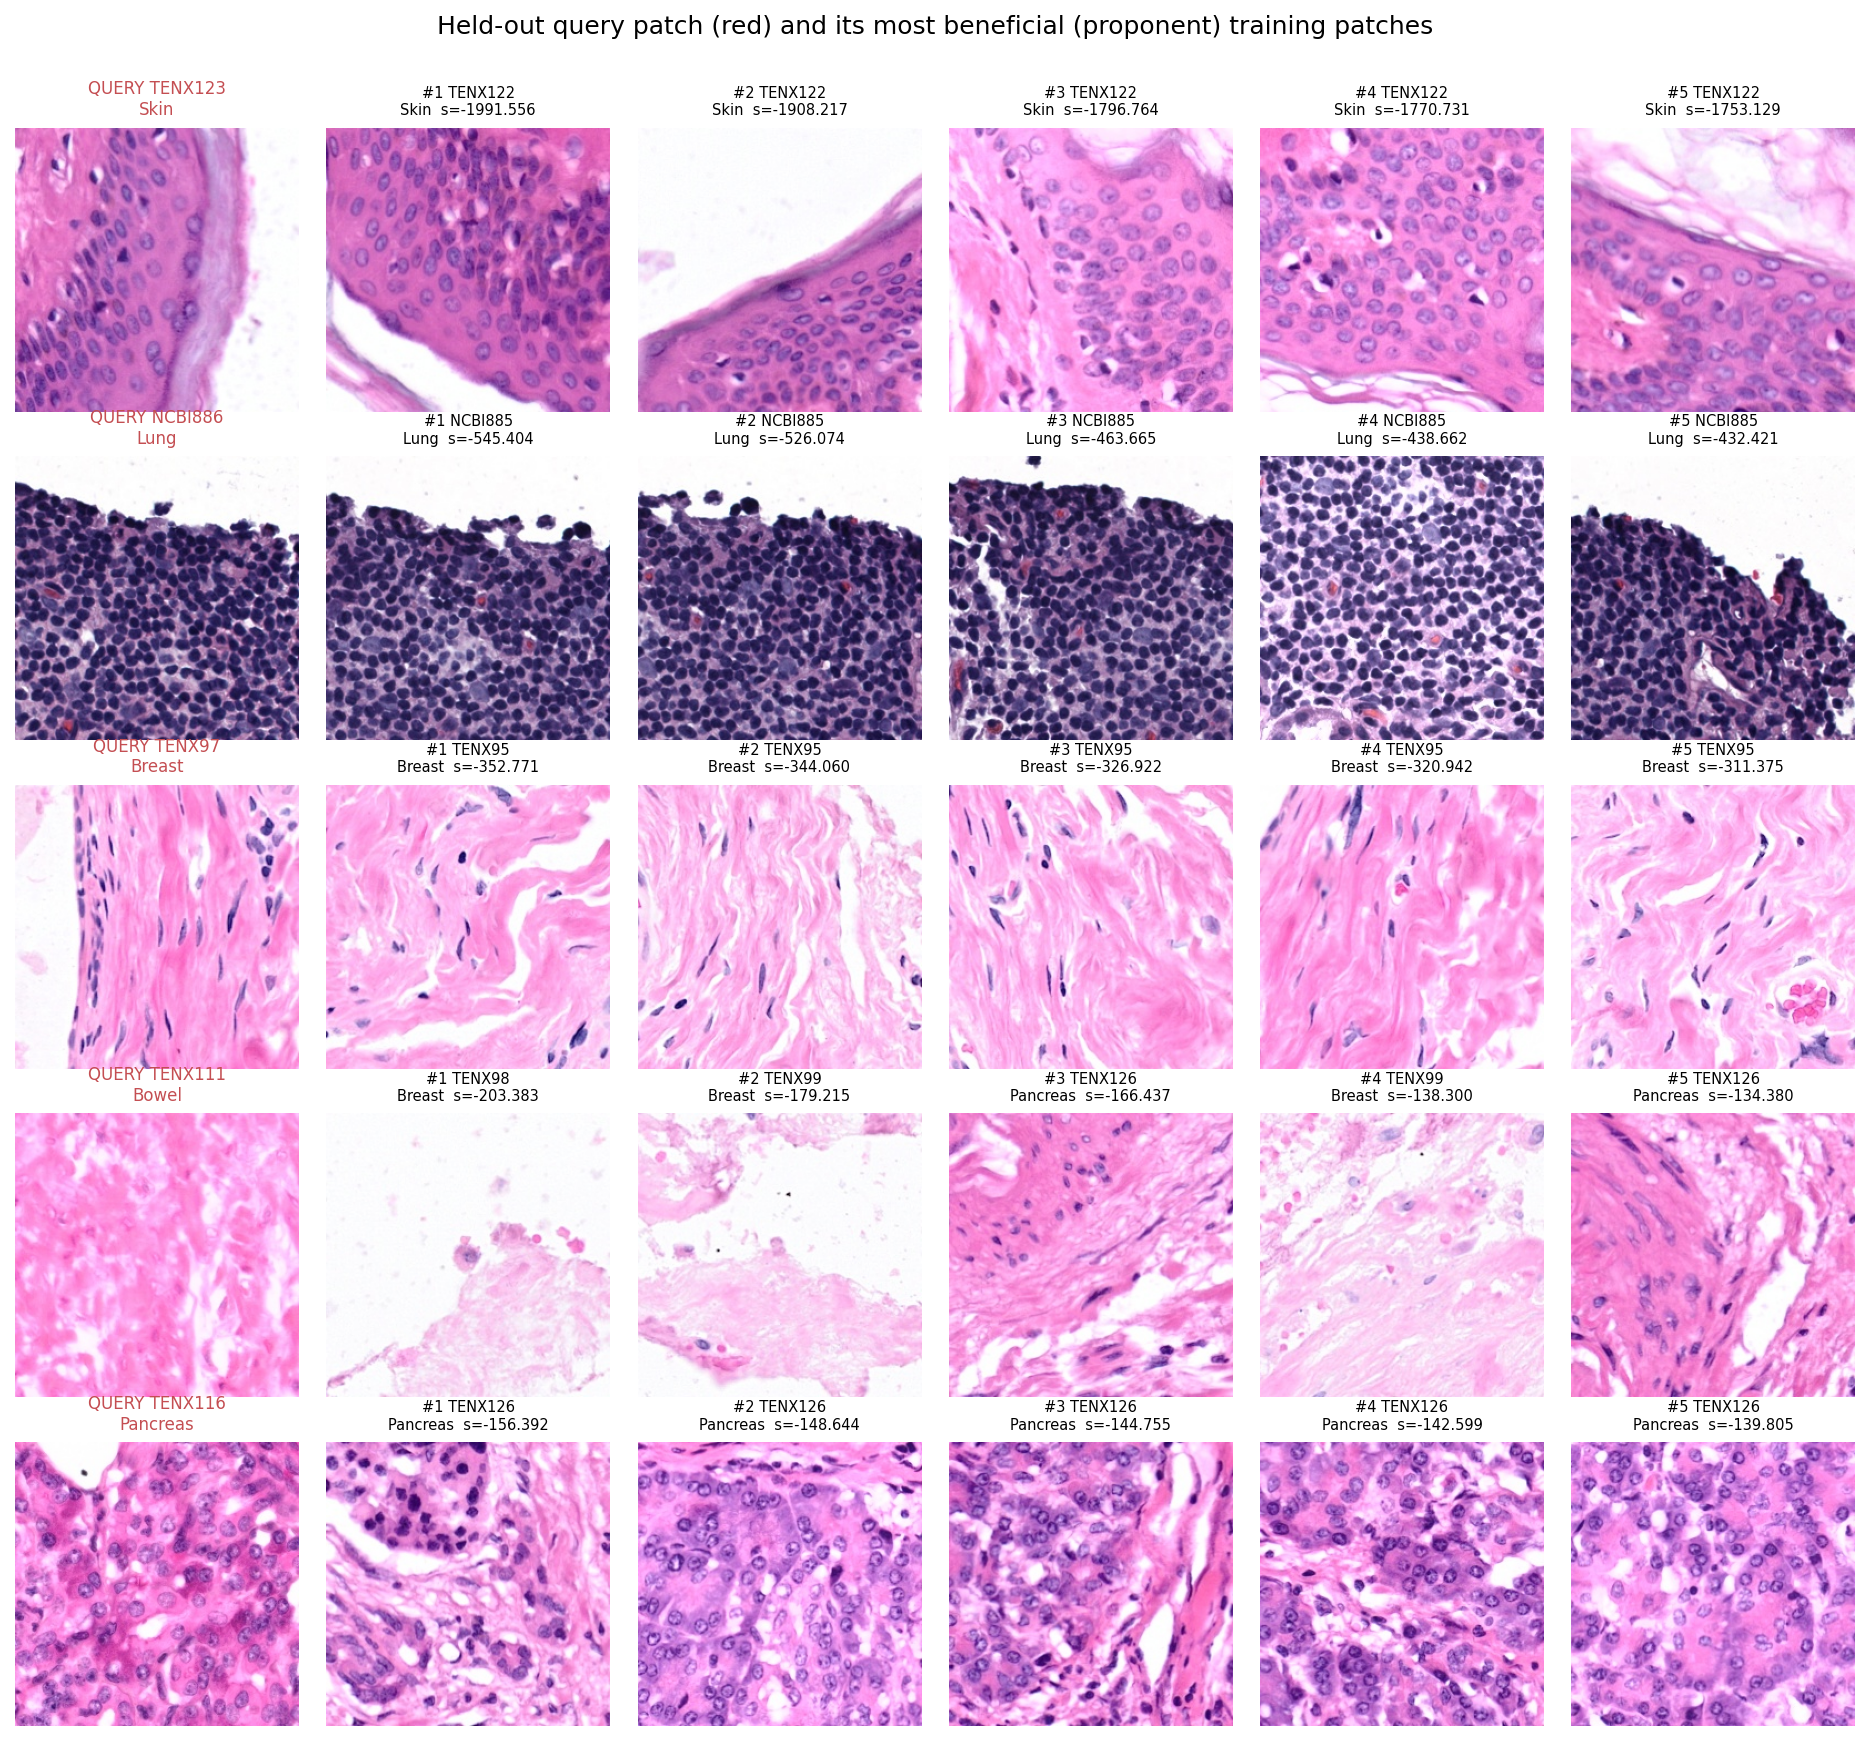
\includegraphics[width=0.66\linewidth]{influence_qualitative.png}
  \caption{Held-out query patch (red, leftmost) and its top beneficial proponent
  training patches per row; same-tissue morphological twins dominate, while bowel
  retrieves breast and pancreas stroma.}
  \label{fig:influence_qual}
\end{figure}

The magnitude of these scores is worth reading carefully, because ranks here are
defined by influence rather than by feature distance
(Figure~\ref{fig:influence_score}). Lists are sorted by score descending, so
rank $1$ is a query's \emph{least} beneficial scored candidate. The median of
those rank-$1$ scores is $-3.8$ (left), already on the beneficial side of zero,
which means that for a typical held-out query essentially the entire scored
shortlist is signed beneficial and outright harmful candidates are the exception.
The right panel shows the median and $10$--$90$ percentile band of the score at
each rank position once a query's $10{,}000$ candidates are sorted. It is
therefore a sorted quantile profile of one distribution: its monotone descent is
guaranteed by the sorting and carries no information about feature-space
proximity or about how deep a kNN pool needs to reach. What it does report is the
shape of that distribution. The bulk of candidates sit in a shallow band around
the median, while the final decade of ranks steepens sharply, the median reaching
about $-22$ and the $10$th percentile falling below $-60$. Strongly beneficial
influence is thus concentrated in a small minority of patches rather than spread
evenly over the shortlist, which is why the tissue attributions above are read
from the bottom-$10$ proponents per query.

\begin{figure}[!htbp]
  \centering
  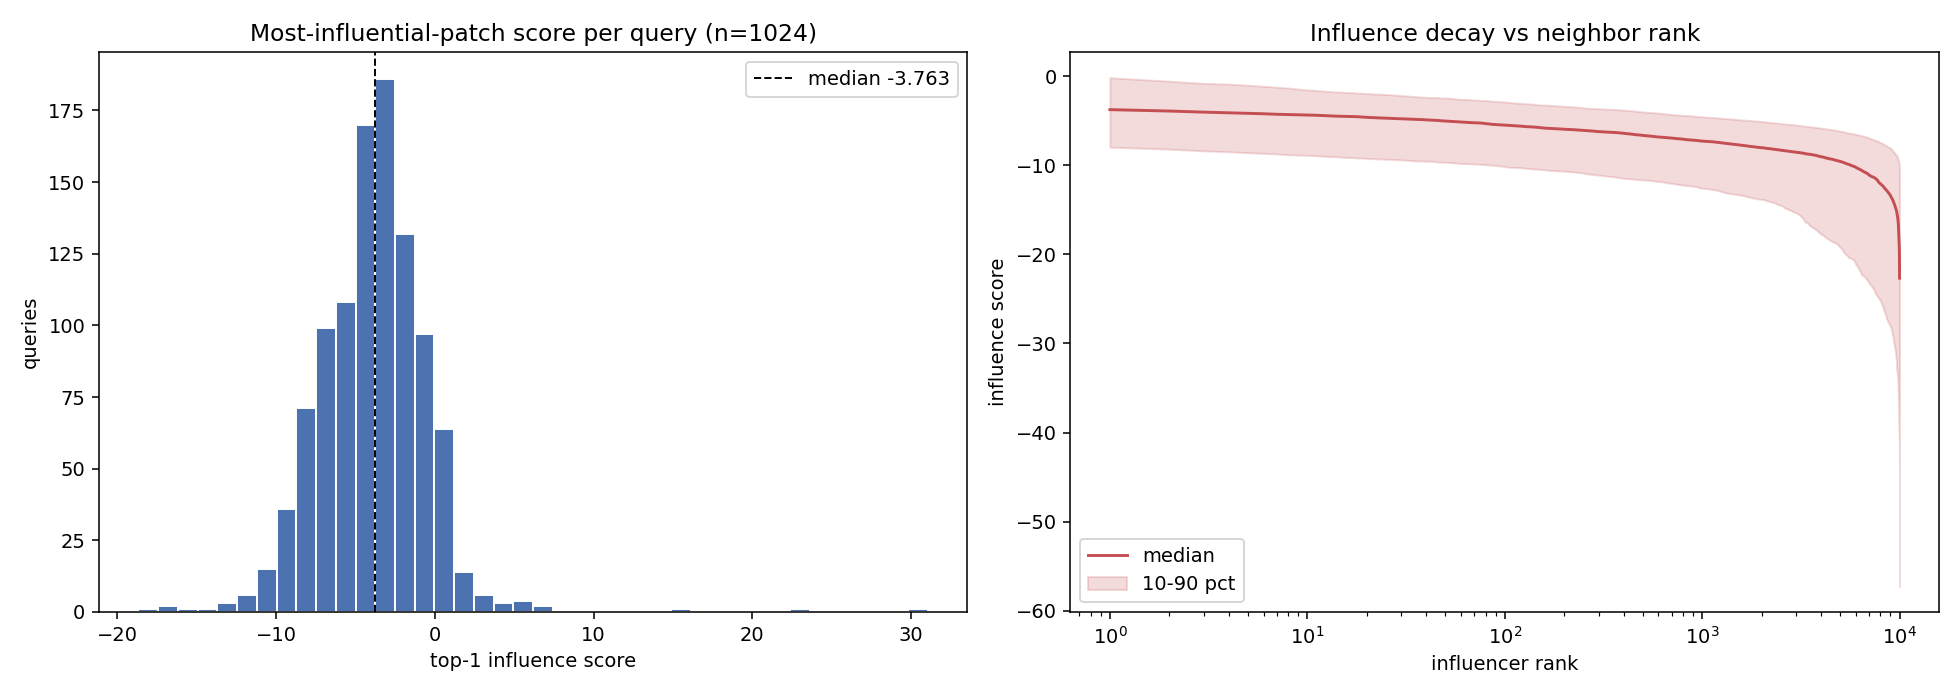
\includegraphics[width=0.9\linewidth]{influence_score_geometry.png}
  \caption{Influence score geometry over 1{,}024 held-out queries
  ($\lambda=0.01$, $k=10{,}000$, raw scores). Left: distribution of each query's
  rank-$1$ (least beneficial) influence score, median $-3.8$, already on the
  beneficial side of zero. Right: median and $10$--$90$ percentile band of the
  score at each rank position after sorting each query's candidates by influence.
  Ranks are defined by the score itself, so this is a sorted quantile profile of
  the score distribution and its monotone descent is a property of the sorting,
  not evidence about feature-space proximity; the sharp steepening in the last
  decade shows that strongly beneficial influence is confined to a small minority
  of candidates.}
  \label{fig:influence_score}
\end{figure}

\section{Clinical Applications}

\subsection{Astra predicts trastuzumab response}
\label{sec:trastuzumab}

Having shown that Astra recovers spatial expression from histology, we now hold
it frozen and ask whether that H\&E-derived expression carries clinical signal in
cohorts where spatial transcriptomics was never measured, beginning with
treatment response. We use trastuzumab (anti-HER2) response in HER2-positive
breast cancer on the Yale cohort (85 pre-treatment patients, 36 responders and
49 non-responders), labeled by pathologic response versus residual
disease~\cite{farahmand_trastuzumab}. Astra stays frozen. Within each patient's
tumor ROIs (Methods~\ref{met:preproc}) it detects cells and predicts their expression tile by tile, giving a
stack of up to roughly 512 tiles across the 1{,}656-gene output panel per
patient.

Rather than pooling every cell into a single slide-level vector, we keep the tile
structure. Each tile is collapsed to a mean expression profile, and each gene is
then summarized across the patient's tiles three ways
(Methods~\ref{met:downstream}): the mean, the median, and the 90th percentile, a
hotspot term weighting the most strongly expressing tiles. Each summary yields
1{,}656 features per patient. In each outer 5-fold split, the 17 test patients
remain untouched. The feature budget is fixed at $K=5$; what the inner stratified
5-fold cross-validation over the 68-patient development set chooses is which
summary family to use, by standardizing and ranking genes by response correlation
on each inner training split, fitting an L2-regularized logistic regression on the
top five, and scoring the held-out inner folds. We then refit the selected model
on all 68 development patients before predicting the 17 test patients.

\begin{figure}[!htbp]
  \centering
  \begin{subfigure}{0.48\linewidth}
    \centering
    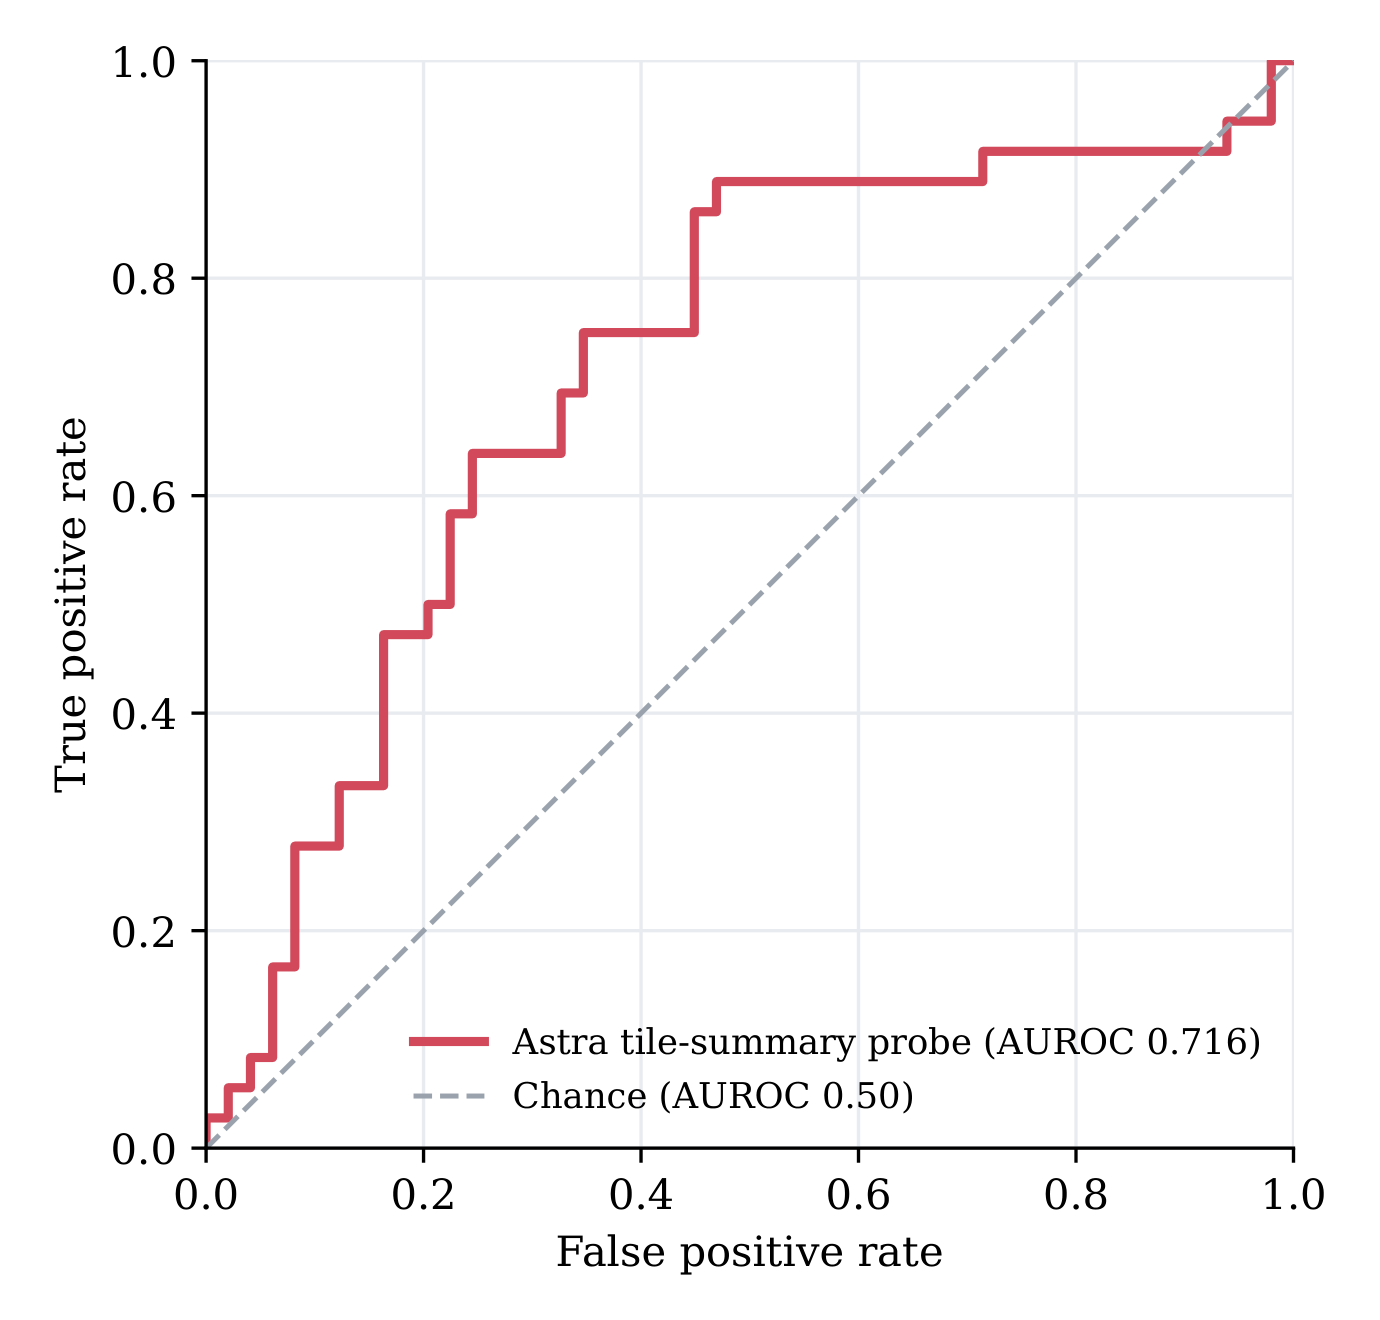
\includegraphics[width=\linewidth]{her2_roc.png}
    \caption{ROC.}
    \label{fig:her2}
  \end{subfigure}
  \hfill
  \begin{subfigure}{0.48\linewidth}
    \centering
    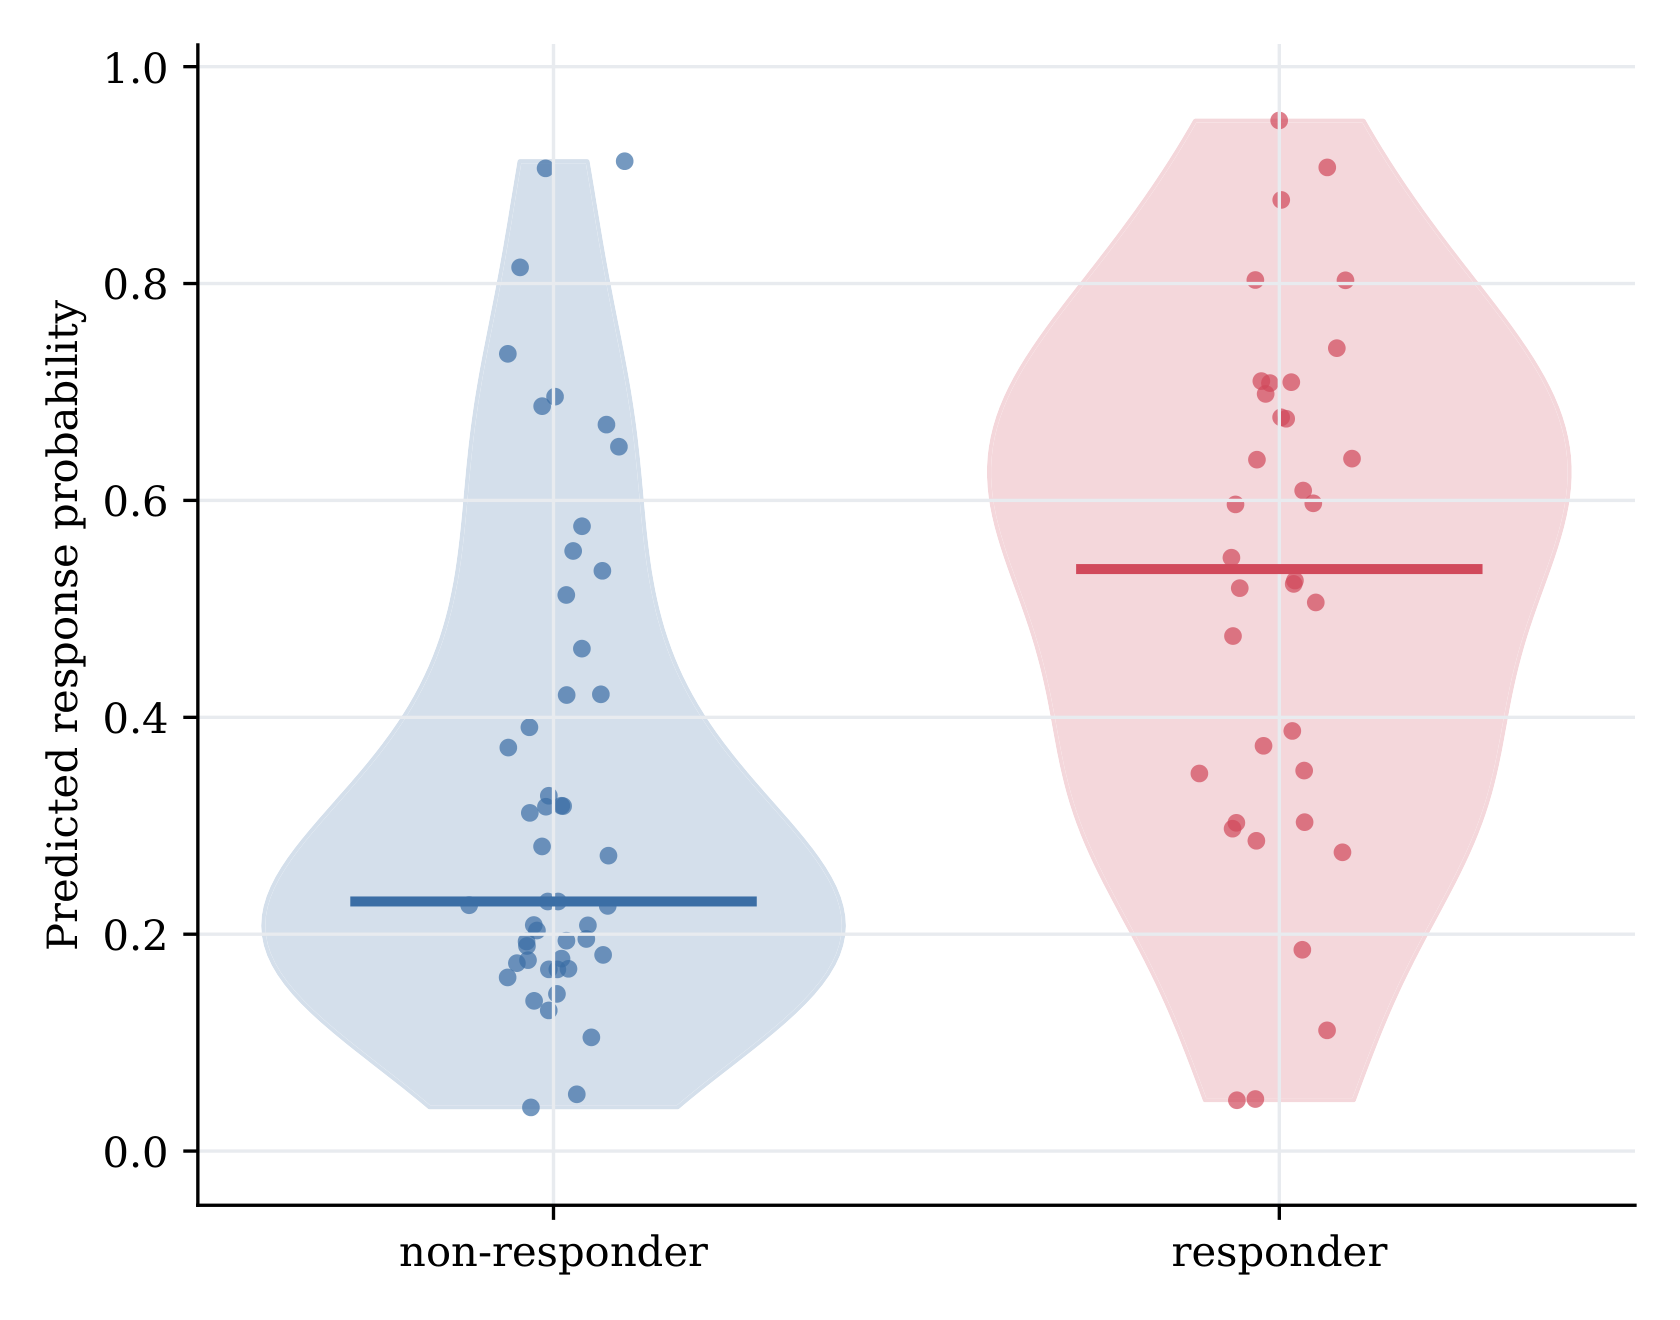
\includegraphics[width=\linewidth]{her2_violin.png}
    \caption{Predicted probability by status.}
    \label{fig:violin}
  \end{subfigure}
  \caption{Trastuzumab response from Astra-derived tile-summary features
  ($n=85$): ROC (AUROC 0.716) and out-of-fold probabilities.}
  \label{fig:her2_panel}
\end{figure}

Evaluated with repeated stratified 5-fold cross-validation (50 repeats) on
averaged out-of-fold probabilities, this nested selection
reaches AUROC 0.716 (95\% CI 0.60--0.83 by $2000\times$ bootstrap) against a 0.42
response prevalence (Figure~\ref{fig:her2}). The inner
cross-validation chose the hotspot (P90) summary in 230 of the 250 outer folds,
the mean in 14 and the median in 6. The out-of-fold probabilities separate the
two groups: responders receive a median predicted probability of 0.54 (IQR
0.34--0.70) against 0.23 (IQR 0.18--0.46) for non-responders, with group means of
0.52 and 0.34 (Figure~\ref{fig:violin}). The difference from prior work
is one of supervision: on this same cohort, Farahmand et al.\ trained an
end-to-end Inception-v3 CNN directly on the response label and reported roughly
0.80 slide-level AUROC~\cite{farahmand_trastuzumab}, whereas Astra's
image-to-expression model was optimized only to predict expression, without
task-specific fine-tuning on the response label; only the lightweight linear
probe is trained on it.

\begin{figure}[!htbp]
  \captionsetup{skip=3pt}
  \centering
  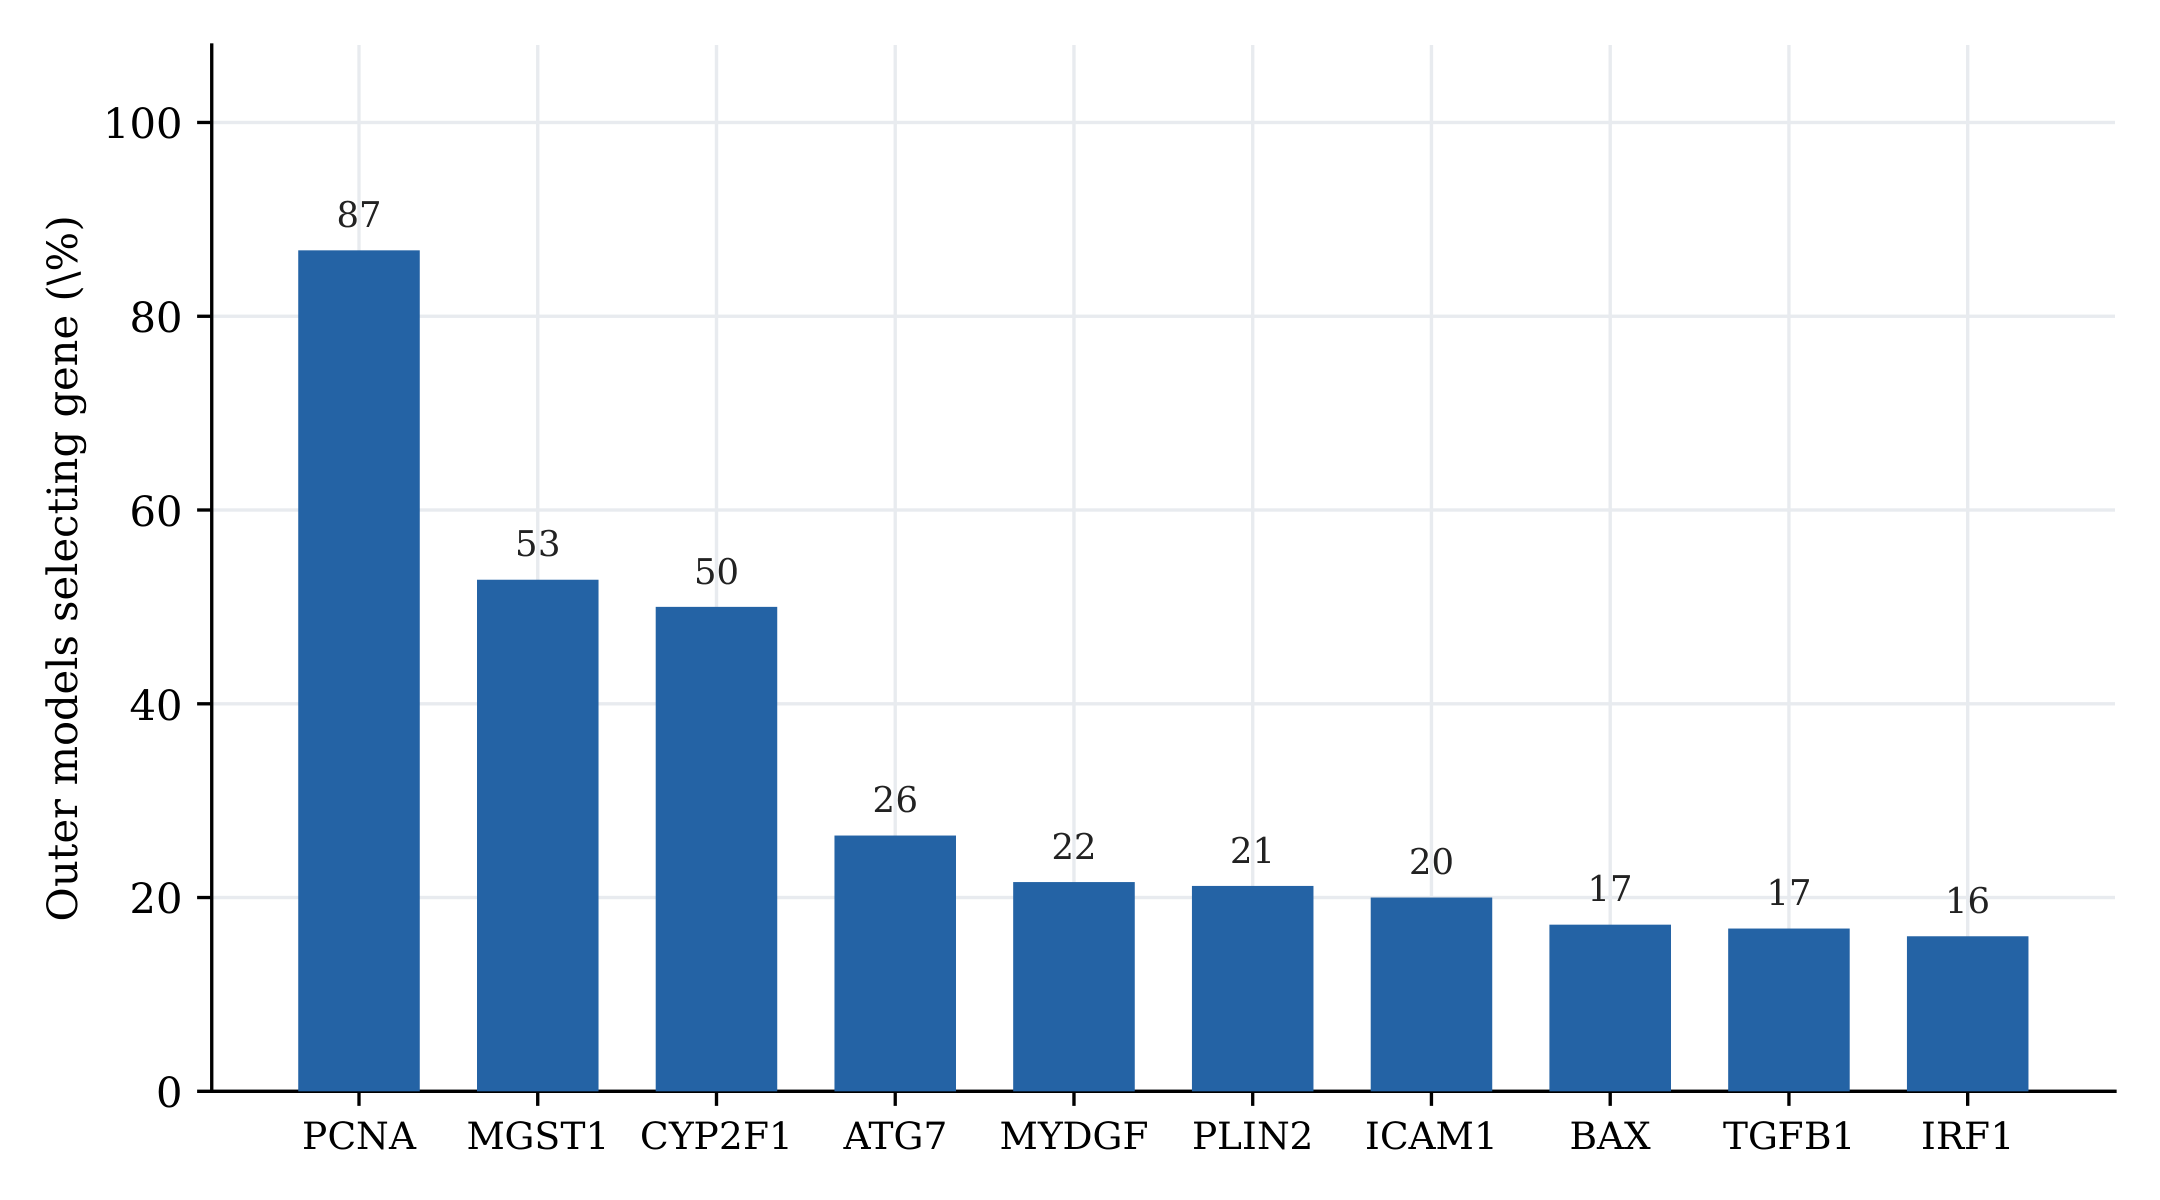
\includegraphics[width=0.72\linewidth]{her2_gene_union.png}
  \caption{Top-10 genes by selection frequency: fraction of the 250
  outer models (5 folds $\times$ 50 repeats) retaining each gene within its
  five-feature budget.}
  \label{fig:her2_gene_union}
\end{figure}

Because the classifier is linear and its selection occurs entirely inside the
training data, we can inspect which features remain stable without using test
labels. Within the five-feature budget a small set of genes recurs: PCNA is
retained by 217 outer models (87\%), followed by MGST1 (132, 53\%) and CYP2F1
(125, 50\%), with the remaining genes each entering fewer than a third of models
(Figure~\ref{fig:her2_gene_union}). The inner loop preferred the P90 summary in
230 of the 250 models, but we do not read that as evidence that heterogeneity
carries the signal: across this cohort the three summary families are
near-duplicates for these genes ($r\ge0.91$), so the preference is marginal.

All three genes are elevated in non-responders, a direction the literature
supports for one of them. MGST1 is a membrane-bound
glutathione transferase that conjugates glutathione to electrophiles, reduces
lipid hydroperoxides, and represses ferroptosis; its overexpression in MCF7
breast-cancer cells confers resistance to several cytostatic drugs and to
oxidative stress~\cite{mgst1_ferroptosis}, so enrichment in tumors that fail to
clear is the expected direction for a detoxification program. PCNA is the
sliding-clamp processivity factor for DNA polymerase; beyond its role as a
proliferation marker it marks aggressive tumor features and poor prognosis in
breast cancer~\cite{pcna_prognosis}, and it is named among the DNA-repair and
damage-response genes differentially expressed in SKBR3 cells driven to
trastuzumab resistance~\cite{pcna_trastuzumab_resistance}.
CYP2F1 is a lung-selective
cytochrome P450 with no established role in breast tissue~\cite{cyp2f1_lung}, and
its recurrence most plausibly reflects structure in predicted expression rather
than a resistance mechanism.

The directions above are univariate associations that do not adjust for one
another.

Response here was predicted without any trastuzumab-specific training of the
expression model: the same frozen Astra supplies the features and only a small
linear probe is fit on the labels. This is the point of routing clinical
prediction through predicted expression rather than training a bespoke
supervised model per task. That expression is a shared substrate, so as the base
model improves from aggregated spatial transcriptomics across more patients, its
predictions become more accurate and every downstream readout built on them
(response here, survival and MSI in the sections that follow) improves at once,
with no new task-specific labels. The clinical results that follow lean on
exactly this transfer.

\subsection{Astra predicts survival risk in luminal breast cancer}
\label{sec:survival}

Trastuzumab response used Astra's expression to predict a treatment endpoint; we
next ask whether the same frozen model carries prognostic signal for a different
clinical outcome and cohort. Overall survival in luminal breast cancer is a
natural test: molecular expression stratifies risk in ways morphology alone does
not make obvious~\cite{luminal_markers}, yet measuring it at single-cell spatial
resolution is rarely feasible at cohort scale. On 772 ER-positive TCGA-BRCA
patients with matched diagnostic H\&E and overall survival (97 deaths, 675
censored; median follow-up ${\sim}865$ days), we retain the 1{,}000 most
tissue-dense tiles per patient (Methods~\ref{met:preproc}), run frozen Astra to predict a 1{,}656-gene
profile at each decoded cell, and average those predictions into one
pseudobulk vector (Methods~\ref{met:downstream}). Repeated 5-fold cross-validation (50 repeats) ranks genes by
survival association within each training fold and fits a multivariable Cox
model on the top 5 genes, the same fixed budget used for the other two tasks,
and only
held-out patients are scored, yielding a pooled concordance index of 0.603
(95\% CI 0.53--0.67).

\begin{figure}[!htbp]
  \centering
  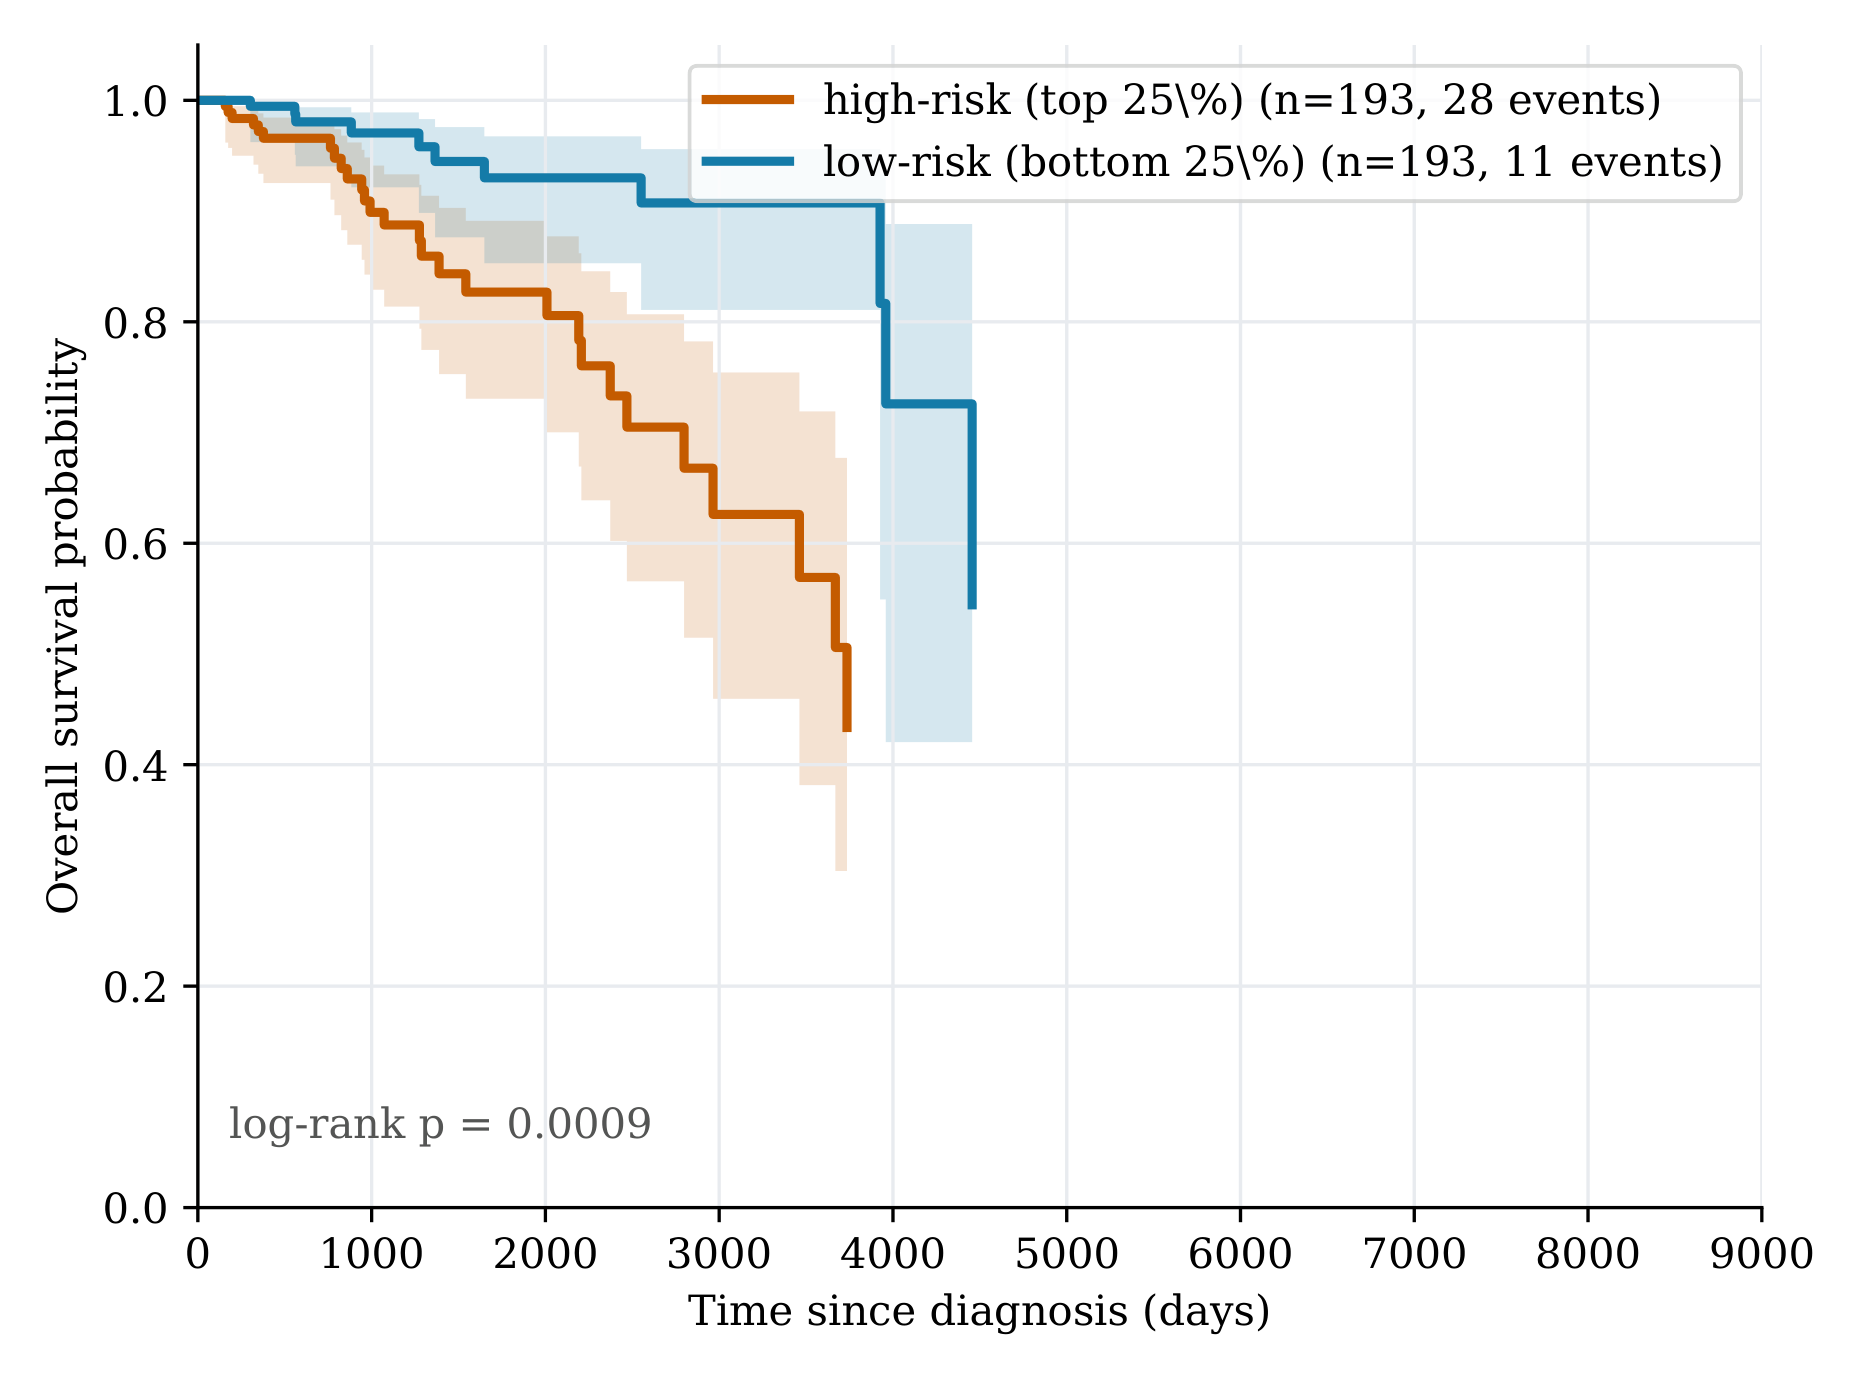
\includegraphics[width=0.68\linewidth]{km_survival_quartiles.png}
  \caption{ER-positive TCGA-BRCA survival for the top and bottom
  cross-validated Astra risk quartiles ($n=193$ each; two-sided log-rank
  $p=0.001$).}
  \label{fig:km_quartiles}
\end{figure}

The separation is sharpest at the extremes of predicted risk: comparing the top
and bottom risk quartiles (193 patients each), the high-risk group has more than
twice as many deaths as the low-risk group (28 vs.\ 11) and the survival curves diverge
early and stay apart (Figure~\ref{fig:km_quartiles}; two-sided log-rank
$p=0.001$). Splitting the full cohort at the median risk preserves the
separation across all 772 patients (386 high vs.\ 386 low; 57 vs.\ 40 deaths;
Figure~\ref{fig:km}; $p=0.022$).

\begin{figure}[!htbp]
  \centering
  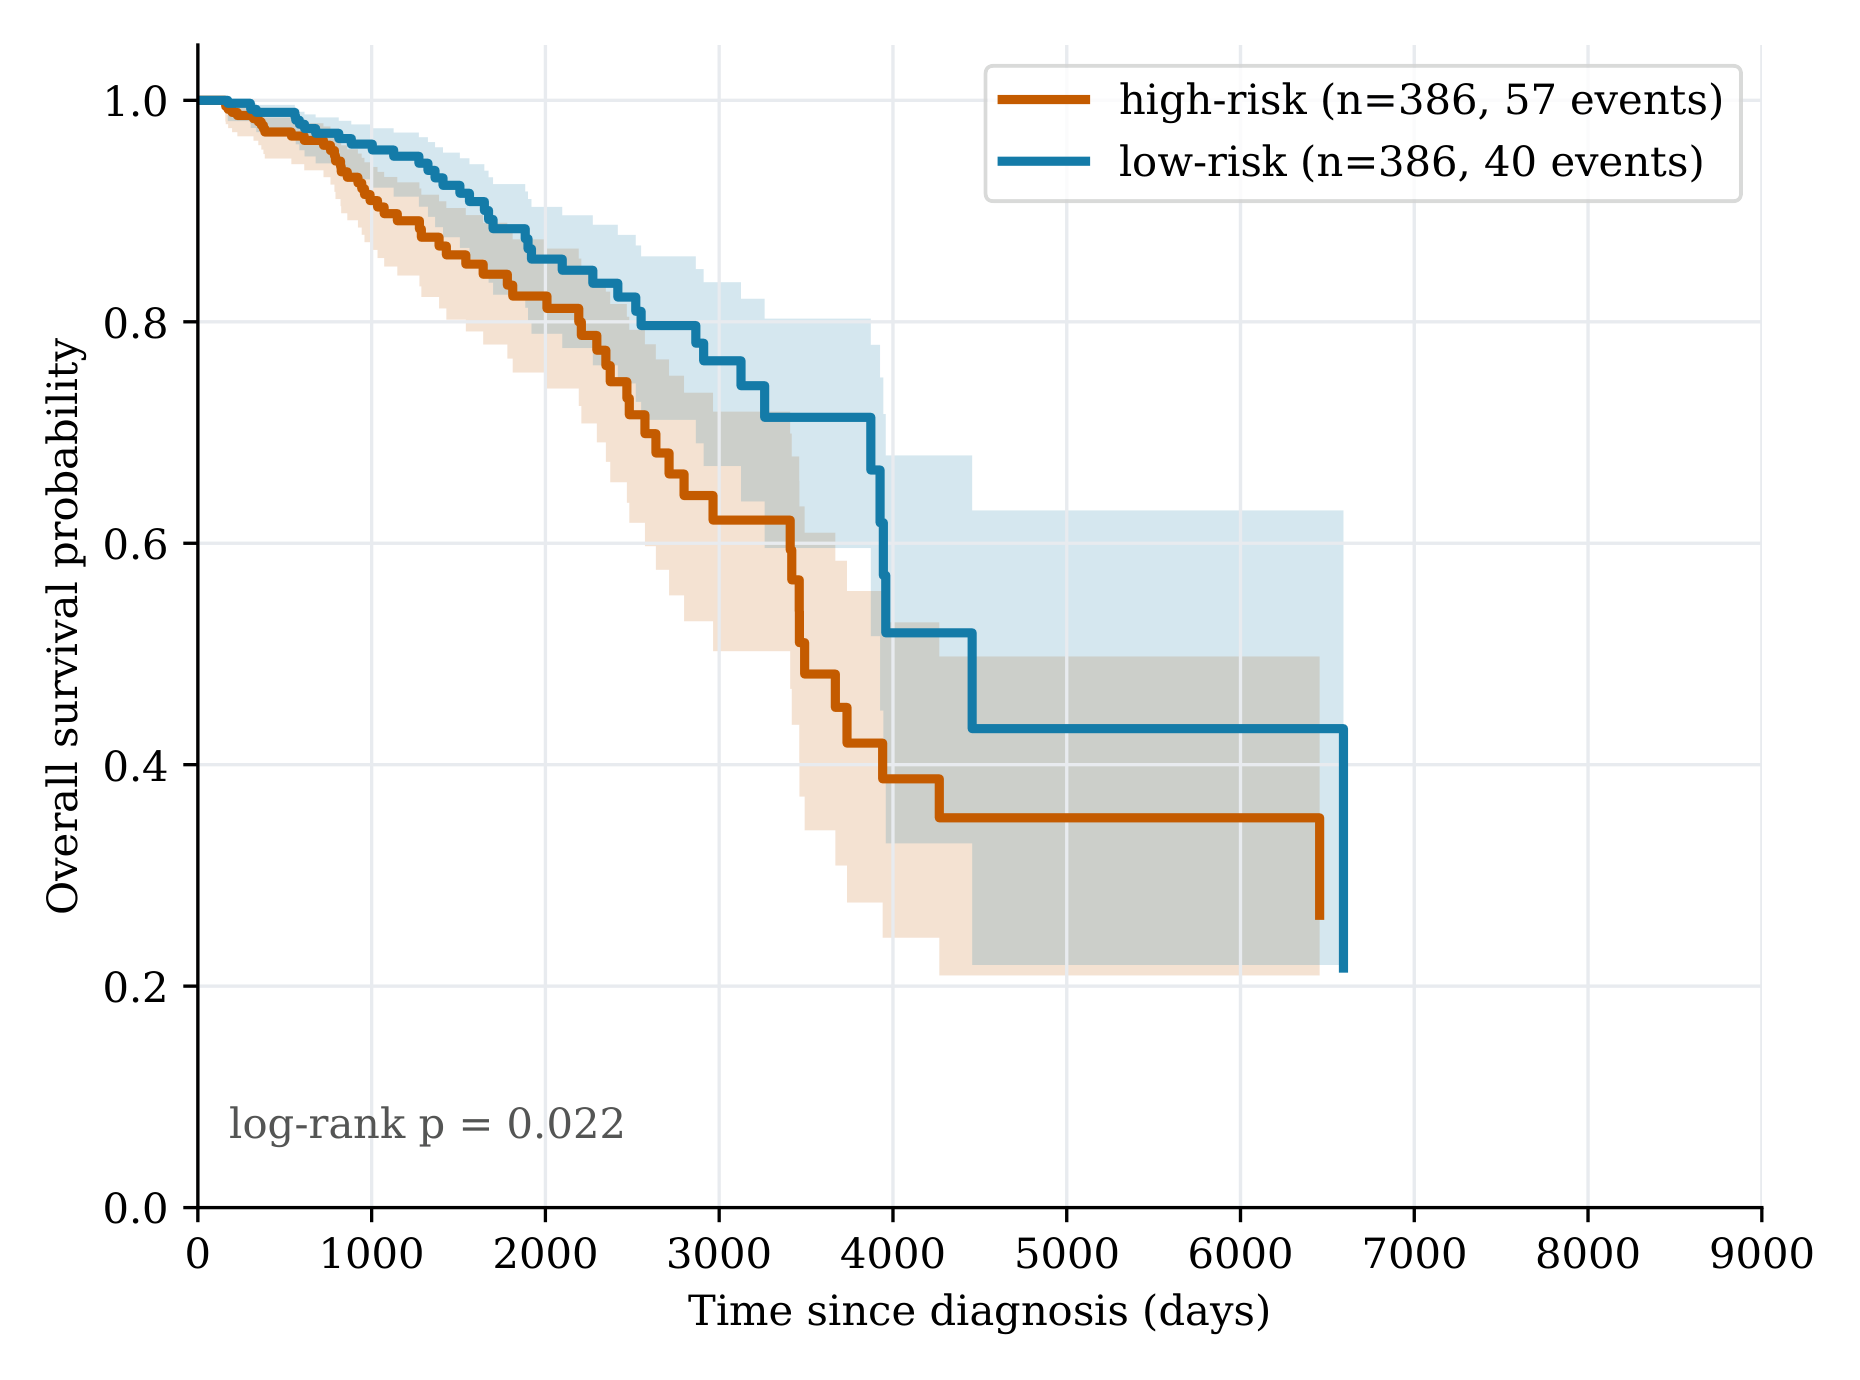
\includegraphics[width=0.68\linewidth]{km_survival.png}
  \caption{ER-positive TCGA-BRCA survival by cross-validated Astra
  risk at the median split ($n=386$ high, $386$ low; two-sided log-rank
  $p=0.022$).}
  \label{fig:km}
\end{figure}

Because gene selection happens entirely inside the training folds, we can read
off which genes recur across the 250 outer models without touching held-out
labels (Figure~\ref{fig:survival_genes}). Because the Cox coefficients are also
recorded, each recurrent gene carries a direction. Two opposing programs emerge.
Cytotoxic and humoral immune markers are consistently protective: KLRC1 (NKG2A;
58\% of folds, mean coefficient $-0.35$), granulysin GNLY ($22\%$, $-0.34$), and
the immunoglobulin heavy chains IGHG4 ($46\%$, $-0.21$) and IGHGP ($32\%$,
$-0.26$). Against them, SERPINB3 ($88\%$, $+0.38$) and the myeloid calprotectin
subunits S100A8 ($58\%$, $+0.25$) and S100A9 ($27\%$, $+0.27$) all carry adverse
risk. Astra therefore recovers a coherent lymphocyte-versus-myeloid survival axis
from H\&E alone, with the sign of each gene consistent across folds.

\begin{figure}[!htbp]
  \captionsetup{skip=3pt}
  \centering
  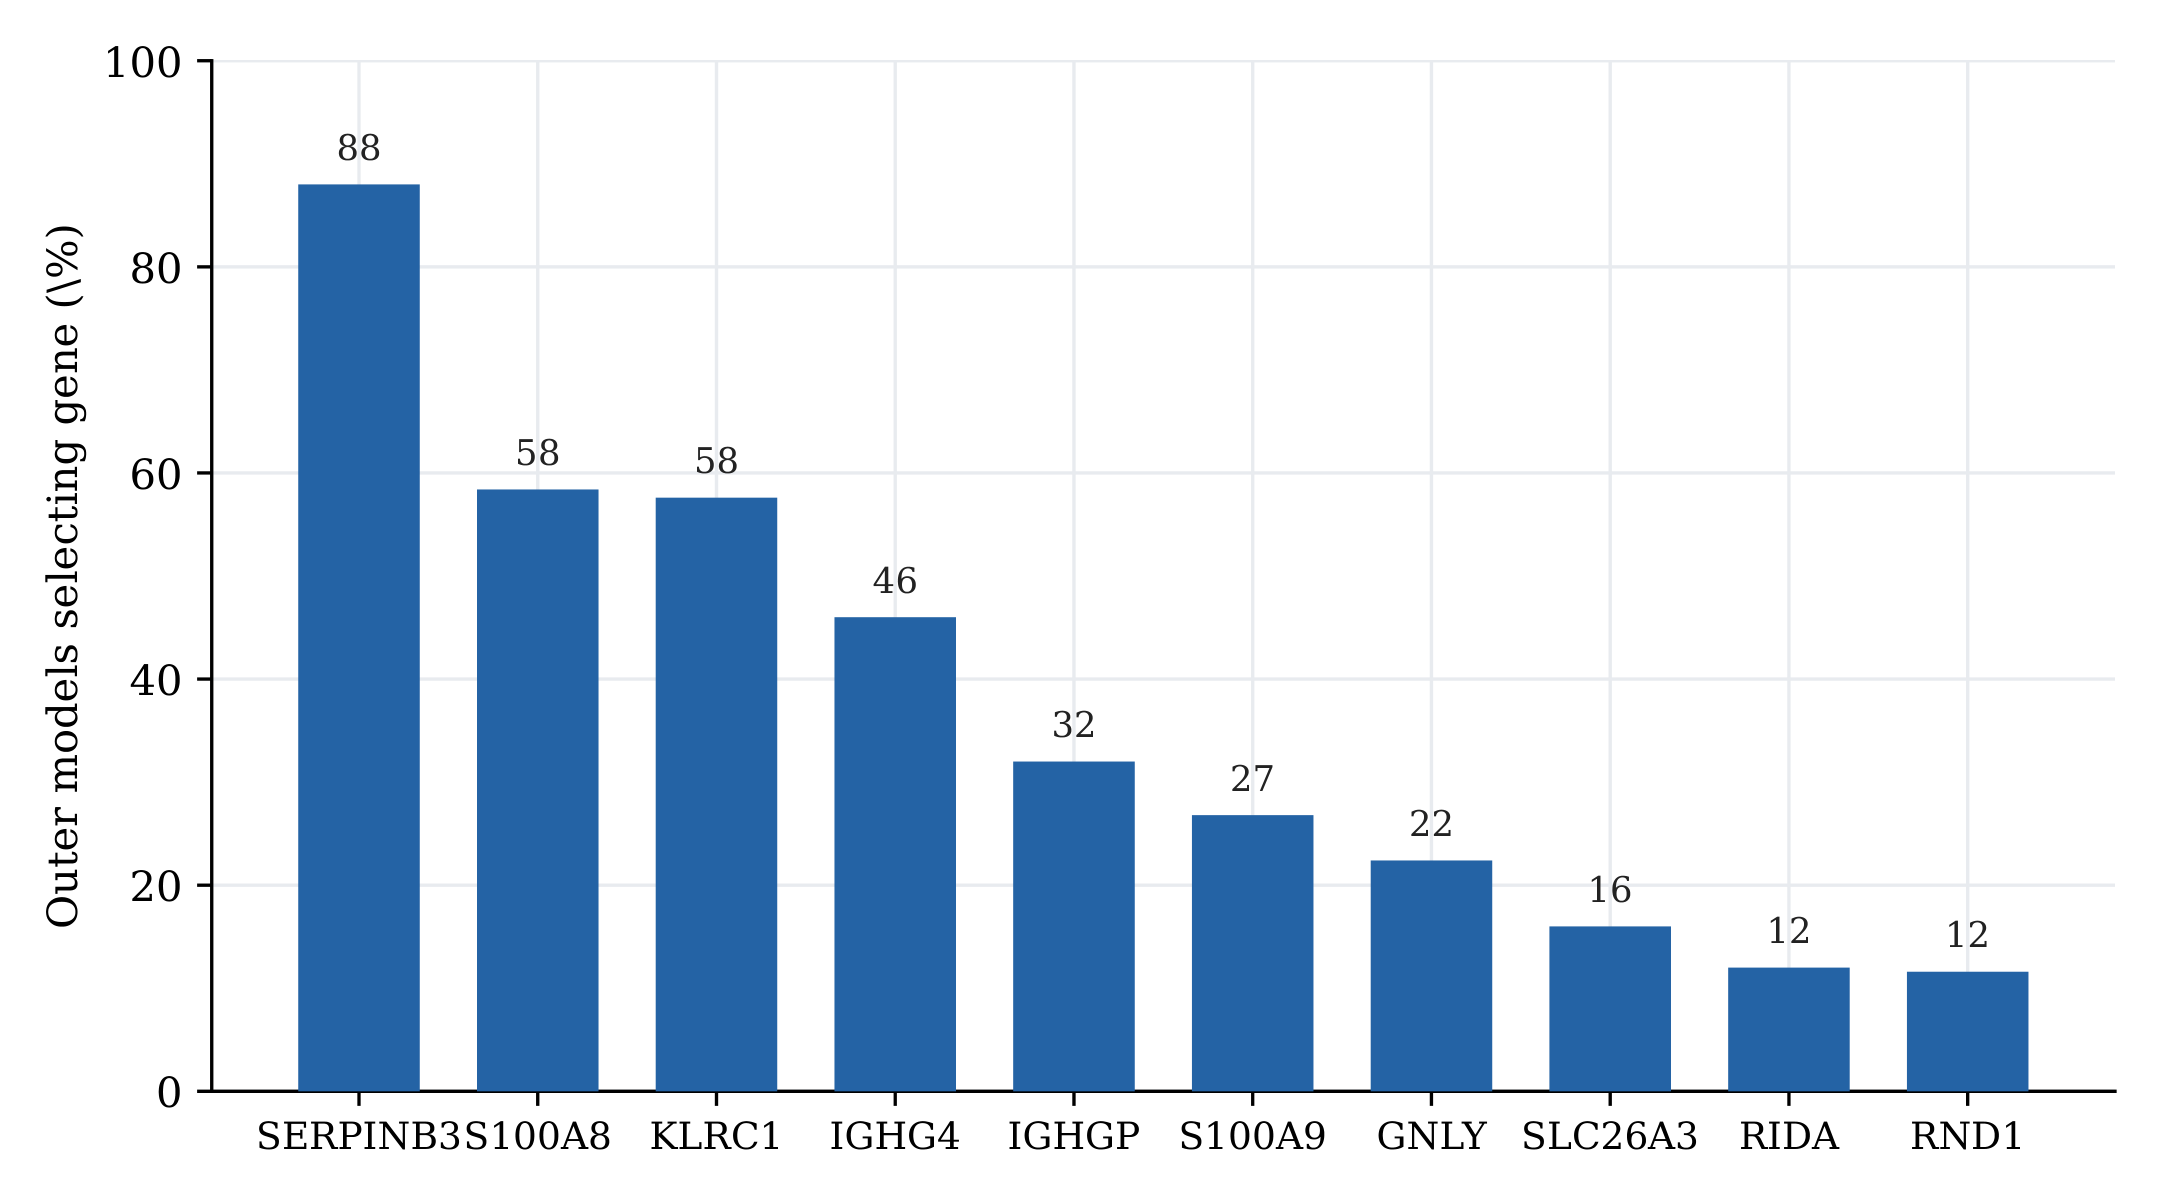
\includegraphics[width=0.72\linewidth]{survival_gene_selection.png}
  \caption{Top-10 genes by cross-validated selection frequency in the
  luminal survival model (fraction of the 250 outer Cox models retaining each
  gene).}
  \label{fig:survival_genes}
\end{figure}

Both directions match documented breast-cancer associations. Immunoglobulin
expression reflecting infiltrating plasma cells is a validated favorable
prognostic marker in breast cancer~\cite{surv_igkc}, which is the direction the
probe assigns to IGHG4 and IGHGP, and dense tumor-infiltrating lymphocytes are a
recognized favorable-prognosis axis~\cite{surv_tils}. Granulysin is a cytolytic
effector released by cytotoxic T and NK cells, and GNLY-positive infiltrate is an
independent predictor of better disease-free survival in breast
cancer~\cite{gnly_til}, matching the protective coefficient the probe assigns it.
On the adverse side, the S100A8/S100A9 heterodimer marks a myeloid inflammatory
program whose elevated expression in tumor cells and stroma is prognostic of
poorer breast-cancer outcome~\cite{surv_s100a8,surv_s100a9}.

SERPINB3, the most frequently selected gene and the one with the largest adverse
coefficient, carries the direction the literature reports. SERPINB3 (SCCA1) is
elevated in high-grade, advanced-stage breast carcinoma and marks worse overall
and recurrence-free survival~\cite{serpinb3_breast}, and in residual tumor after
anthracycline-based neoadjuvant chemotherapy it is an independent prognostic
biomarker of poor outcome (HR 2.1, 95\% CI 1.2--3.8)~\cite{serpinb3_neoadj}.

KLRC1 admits no equivalent mechanistic reading. It encodes NKG2A, an inhibitory
checkpoint receptor whose high expression on NK cells marks exhaustion and immune
evasion, and which is an antibody target because blocking it restores
cytotoxicity~\cite{klrc1_nkg2a}. Its protective coefficient is therefore better
attributed to pseudobulk KLRC1 transcript tracking the abundance of NK and
cytotoxic T cells than to NKG2A signaling itself.

\subsection{Astra can help pre-screen for MSI-H}
\label{sec:msi}

Microsatellite instability (MSI-H) is among the most actionable biomarkers in
oncology: it predicts response to immune-checkpoint inhibitors. Pembrolizumab is
FDA-approved for MSI-H/dMMR solid tumors in a tissue-agnostic
indication~\cite{fda_pembro}, and MSI-H also flags Lynch syndrome for genetic
screening.
Standard testing relies on PCR or immunohistochemistry for mismatch-repair
proteins, so calling MSI from routine H\&E would be a cheap pre-screen, and prior
deep-learning work has shown histology carries this signal~\cite{kather_msi}.
Our test is deliberately strict: the image-to-expression model receives no
task-specific fine-tuning on MSI. It is trained only on HEST-1k spatial
transcriptomics, with no TCGA data and no MSI labels anywhere in that model; only
the linear probe on top sees the label. We run frozen Astra over TCGA colorectal slides
(TCGA-COAD and TCGA-READ; 255 patients, 85 MSI-H), pool predicted per-cell
expression into one pseudobulk profile per patient, and fit only a linear
classifier on top under nested cross-validation (Methods~\ref{met:downstream}; repeated stratified 5-fold
outer CV, 50 repeats), keeping the top 5 AUC-ranked genes per training split and
averaging over the mean and median tile summaries, scored against the
genomic MANTIS label~\cite{mantis}.

\begin{figure}[!htbp]
  \centering
  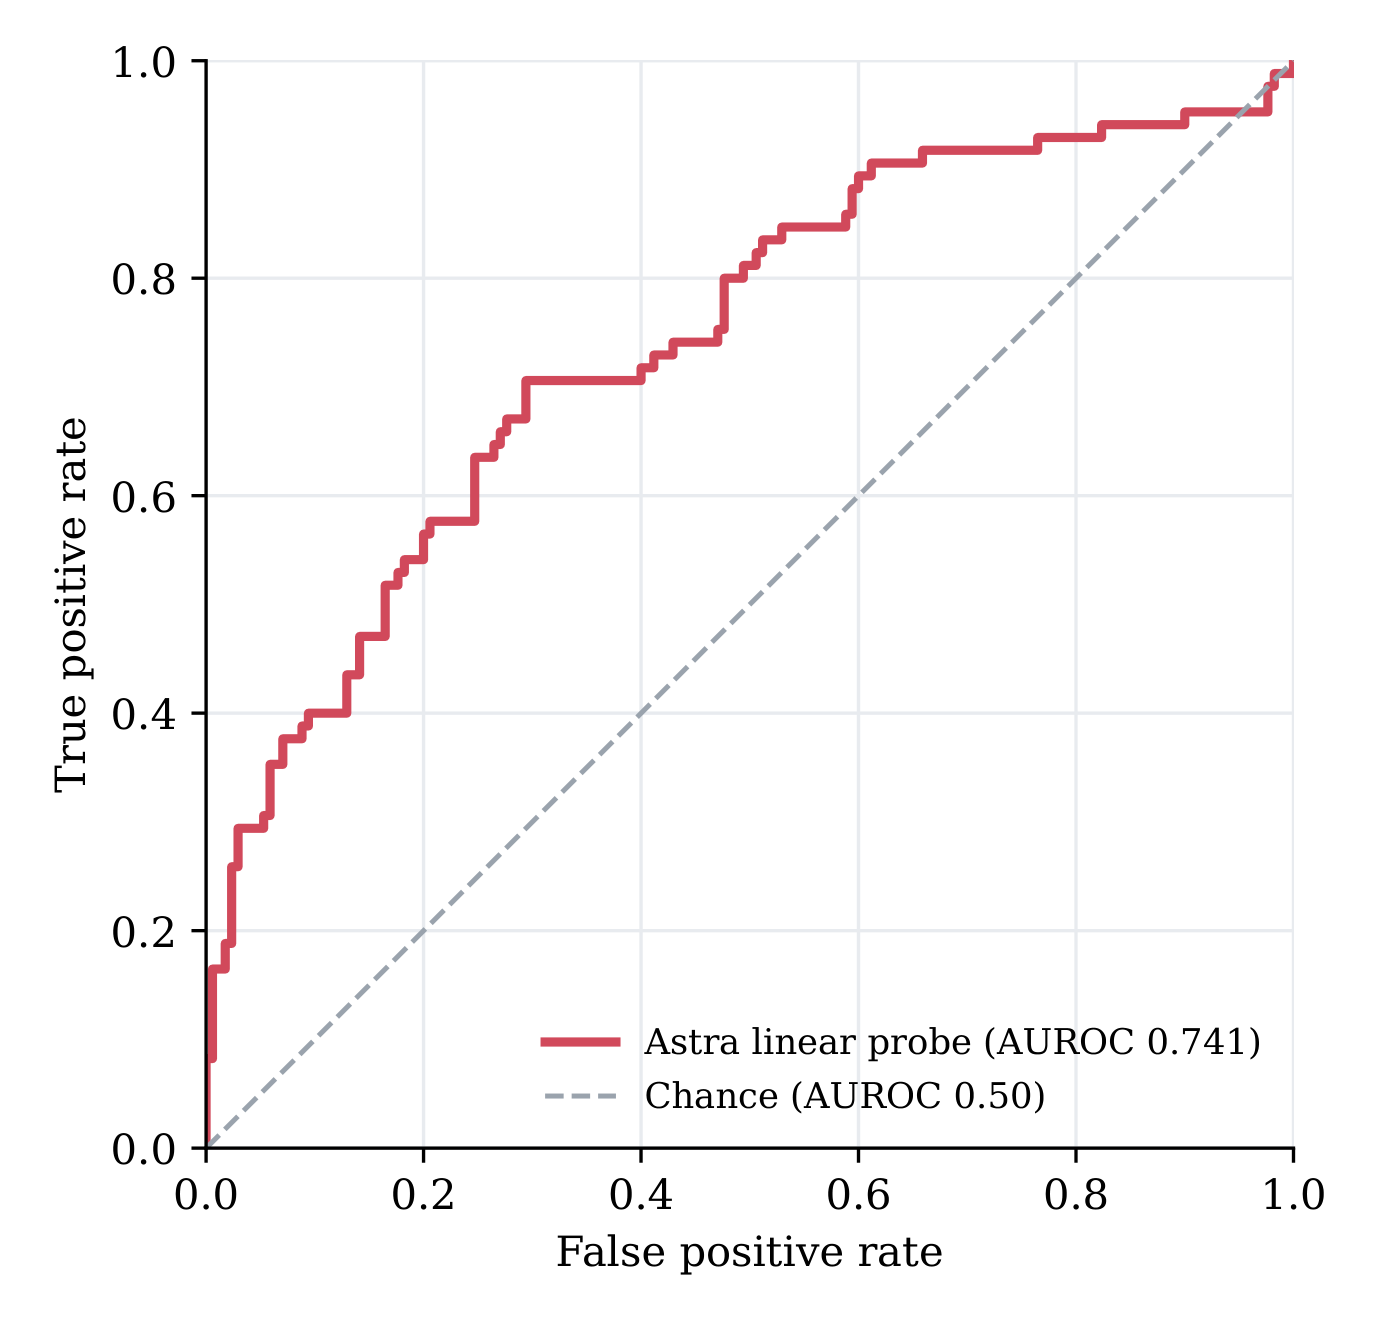
\includegraphics[width=0.5\linewidth]{msi_roc.png}
  \caption{MSI-H detection from Astra-predicted pseudobulk expression
  in TCGA-COAD/READ (AUROC 0.741).}
  \label{fig:msi}
\end{figure}

The linear probe reaches AUROC 0.741 at a cohort prevalence of 33\% MSI-H
(Figure~\ref{fig:msi}).
This is competitive with the within-cohort TCGA models trained end-to-end on MSI
labels (patient-level AUC 0.77--0.84~\cite{kather_msi}; our bootstrap 95\% CI
reaches 0.81). Astra reaches this without any of that
task-specific machinery: it sees no MSI label or TCGA slide in training and fits
only a named-gene linear probe, keeping an interpretability those end-to-end
detectors lack. As argued for trastuzumab (Section~\ref{sec:trastuzumab}),
predicted expression is the shared substrate, so gains to the base model from
aggregated spatial transcriptomics carry over to this task with no new MSI
supervision.

Because the probe is linear and its genes are named, the prediction can be read
directly. Hypermutated, neoantigen-rich MSI-H tumors recruit an inflamed immune
infiltrate~\cite{msi_immune}, and the two most stable features fit that picture.
COTL1 enters essentially every probe (99\%): it is an actin-binding protein of
the ADF/cofilin family that is highly expressed in leukocytes and is required at
the immune synapse, where it protects F-actin from cofilin-mediated
disassembly and supports lamellipodial protrusion during T-cell
activation~\cite{cotl1_synapse}. CXCL5 enters 69\% and is a CXCR2-ligand
neutrophil chemoattractant that is overexpressed in colorectal tumors and
associated with advanced stage, liver metastasis, and poor
prognosis~\cite{cxcl5_crc}. Both are immune-compartment genes, which is the axis
that separates MSI-H from MSS tissue.

Several of the remaining genes have colorectal literature, though none is a
mismatch-repair marker. NMB (74\%) is elevated in colorectal tumors relative to
normal mucosa and is an independent predictor of poor survival, acting through
USP21-stabilized NF-$\kappa$B signaling~\cite{nmb_crc}. MARCKSL1 (64\%) is an
actin-regulatory protein of innate immune cells that is raised in the circulating
extracellular vesicles of metastatic colorectal cancer patients and has been
proposed to separate metastatic from non-metastatic disease~\cite{marcksl1_crc}.
HIST1H4C (64\%) is a replication-dependent histone transcribed in S phase and so
reads as a proliferation correlate. These mark tumor aggressiveness and immune
content rather than mismatch repair.

The remaining features admit no such support. TSC22D1 (52\%) and STRADB (47\%)
have no established colorectal or mismatch-repair association, and the recurrent
selection of the melanocytic genes TYR (62\%) and PMEL (11\%) in colorectal
tissue is more plausibly a panel artifact than a biological finding.

\begin{figure}[!htbp]
  \captionsetup{skip=3pt}
  \centering
  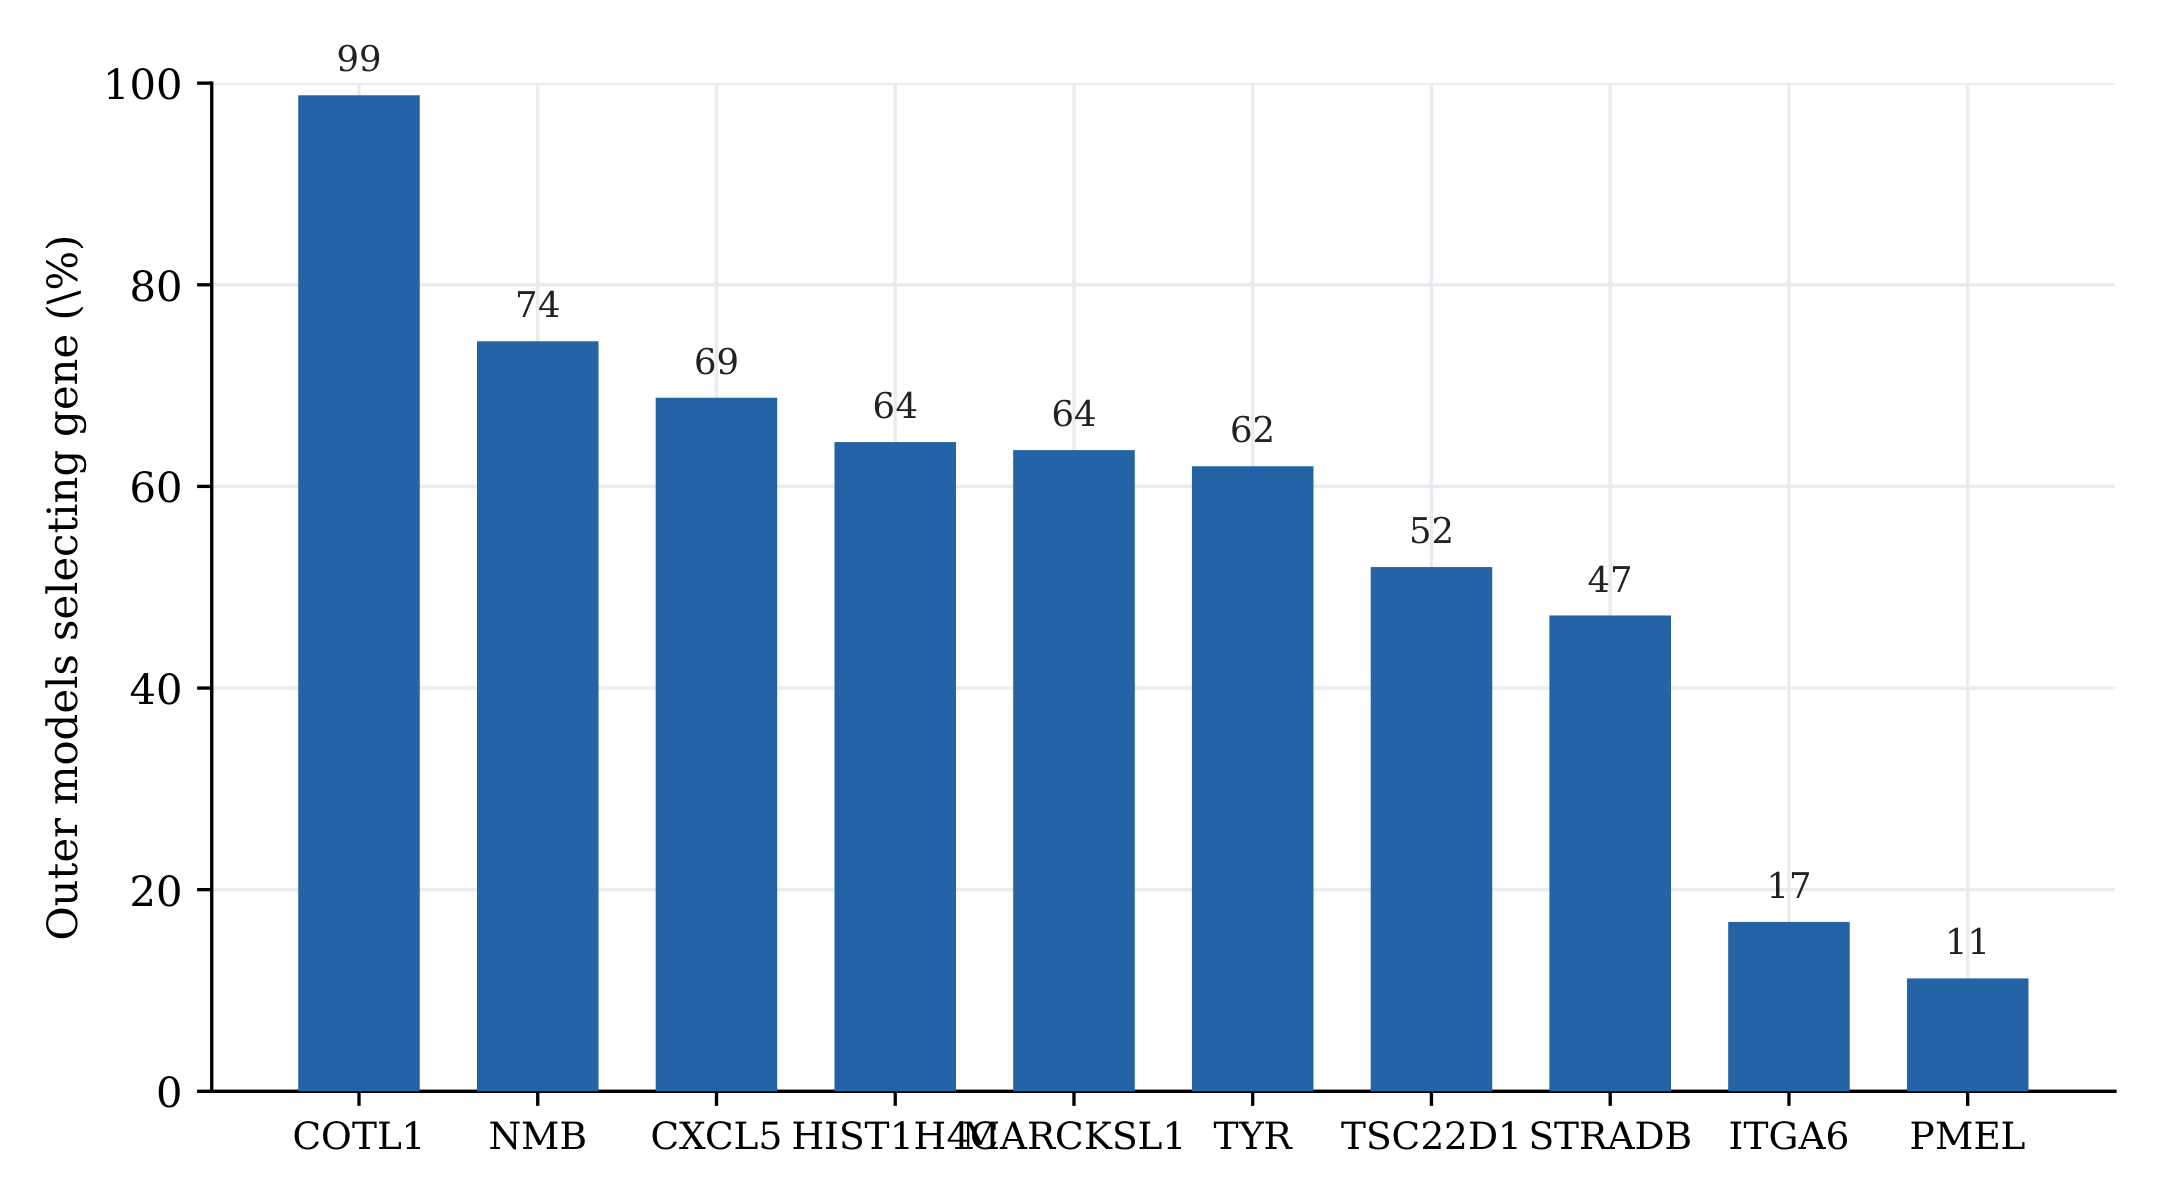
\includegraphics[width=0.72\linewidth]{msi_gene_selection.png}
  \caption{Top-10 genes by cross-validated selection frequency in the
  MSI-H probe. Each bar is the fraction of the 750 fitted probes (250 outer
  models $\times$ 3 regularization settings) in the gene's dominant summary
  family that retain it.}
  \label{fig:msi_genes}
\end{figure}

A frozen, cross-domain expression model, without task-specific fine-tuning on
MSI, therefore recovers an established clinical biomarker through an
interpretable, named-gene route rather than an opaque classifier, and identifies
the genes responsible. Two limits apply: these results are cross-validated within
TCGA rather than externally validated, and the 33\% MSI-H prevalence here is
enriched relative to the roughly 15\% observed clinically.

\section{Discussion}

Astra establishes a general architecture for learning single-cell molecular
representations from routine histology. By jointly inferring cellular position
and expression, it removes the requirement for a spatial assay or separately
matched segmentation at inference. The same frozen representation transfers
from expression recovery to pathologist-annotated cell composition,
treatment-response prediction, survival stratification, and MSI-H pre-screening.
Together, these findings suggest that
spatial-expression supervision can produce histologic representations with
clinical utility across treatment response, prognosis, and biomarker screening.
Prospective, multi-institutional validation is required before deployment.

This separation between a general image-to-expression model and a lightweight
task-specific model is important. A single frozen model could be run
retrospectively over existing pathology archives, after which small labeled
cohorts could be used to test response, prognosis, or biomarker hypotheses
without retraining Astra for every endpoint. Single-cell output also
preserves regional heterogeneity that slide-level embeddings and pseudobulk
measurements can erase. In practice, this could support molecular-test triage,
identify tissue regions for confirmatory profiling, and help prioritize patients
for biomarker-directed studies while retaining a spatial record of the predicted
signal.

One particularly relevant use is clinical-trial enrichment, which we raise as a
hypothesis to be tested prospectively rather than a demonstrated capability. FDA
guidance defines predictive enrichment as selecting patients ``more likely to
respond to the drug treatment than other patients with the condition'' and notes
that this can increase effect size and permit a smaller study
population~\cite{fda_enrichment}. This matters because aggregate trial results
can obscure spatially defined differences in treatment response.
In NeoTRIP, adding atezolizumab did not significantly improve pathologic complete
response overall (48.6\% vs.\ 44.4\%, $p=0.48$), but retrospective imaging mass
cytometry of archived trial tissue found that cellular composition and spatial
organization distinguished immunotherapy-sensitive from resistant
tumors~\cite{neotrip_spatial}. In NSABP B-41, the H\&E-derived DeSTIL spatial
immune signature identified a subgroup with markedly better event-free survival
on trastuzumab than the combination arm (HR 0.09; interaction $p=0.024$), while
signature-negative patients showed no treatment difference~\cite{destil_b41}.
Exploratory analysis of KATHERINE likewise found no T-DM1 benefit in the subgroup
with focal HER2 expression below 30\% (HR 1.21; focal-versus-nonfocal interaction
$p<0.05$), although the subgroup was small and the confidence interval wide
(0.58--2.51)~\cite{katherine_biomarkers}. These retrospective results show how an
aggregate trial effect can conceal treatment-relevant spatial organization. An
inexpensive H\&E-based pre-screen for a response-associated spatial program could
prioritize patients for confirmatory testing or enrollment, potentially
recovering efficacy signals that an unselected trial would dilute. Its near-term
value is as a scalable screening layer that reduces the samples needing costly
molecular assays, not as a determinant of eligibility on its own. More broadly,
Astra shows how inferred single-cell expression can turn routine histology into
a scalable substrate for biomarker discovery, trial enrichment, and clinically
directed molecular profiling.

\section{Methods}
\label{sec:methods}

\subsection{Model architecture}
\label{met:arch}

Astra maps an H\&E patch and a set of cell positions to per-cell gene
expression. Each patch is a $256\times256$-pixel tile resampled to
$0.5\,\mu$m/pixel (a $128\,\mu$m field of view), then bilinearly resized to
$224\times224$ and ImageNet-normalized before the encoder. The image encoder is
a frozen Prov-GigaPath ViT-G/16~\cite{gigapath} with embedding dimension
$1536$; we keep its full token grid, $197$ tokens per patch (one class token and
a $14\times14$ grid of patch tokens), rather than pooling to the class token.

The shared trunk is a four-layer pre-norm transformer over these $197$ tokens
with eight attention heads (head dimension $192$). Each layer normalizes with
root-mean-square norm (RMSNorm~\cite{rmsnorm}),
$\mathrm{RMSNorm}(x)=x/\sqrt{\tfrac{1}{d}\sum_i x_i^2+\epsilon}\;\odot\gamma$,
and uses a gated SwiGLU feed-forward block~\cite{swiglu_shazeer},
$\mathrm{SwiGLU}(x)=W_{\mathrm{down}}\big(\mathrm{SiLU}(W_{\mathrm{gate}}x)\odot
W_{\mathrm{up}}x\big)$ with inner width $4{,}096$, in place of a GELU MLP. Token
position is injected by two-dimensional rotary position embeddings
(RoPE~\cite{rope_su}) applied
to the queries and keys: each head's channels are split in half, one half rotated
by the token's grid column and the other by its row (base frequency $\theta=100$;
the class token is given the identity rotation). Before rotation, queries and
keys are per-head RMSNorm-normalized (QK-norm) for training stability. Concretely,
for query/key vector $u$ at grid position with rotary tables $(\cos,\sin)$,
$\mathrm{RoPE}(u)=u\odot\cos+\mathrm{rot}_{\text{half}}(u)\odot\sin$, and
attention is the usual softmax over $q^{\top}k/\sqrt{192}$. A final RMSNorm is
applied before the heads read from the trunk.

Cells enter as queries. A cell at pixel $(x,y)$ inside the patch is expressed as
a patch-relative coordinate $(dx,dy)\in[-1,1]^2$ and embedded with a
NeRF-style Fourier feature map~\cite{tancik_fourier} using eight frequency bands
$\omega_k=\pi\,2^{k}$ for $k=0,\dots,7$:
\[
\phi(dx,dy)=\big[\sin(\omega_k dx),\cos(\omega_k dx),
\sin(\omega_k dy),\cos(\omega_k dy)\big]_{k=0}^{7}\in\mathbb{R}^{32},
\]
which a linear layer projects to $1536$ and an RMSNorm normalizes. This query
cross-attends (eight heads) to that patch's $197$ image tokens, producing one
$1536$-dimensional feature per cell; the feature is RMSNorm'd and refined by a
residual SwiGLU feed-forward block,
$\mathrm{SwiGLU}(x)=W_{\mathrm{down}}\big(\mathrm{SiLU}(W_{\mathrm{gate}}x)\odot
W_{\mathrm{up}}x\big)$ with inner width $4{,}096$. Because each cell is queried
at its own centroid, there is no nucleus-to-transcript matching step.

Three linear heads read the per-cell feature. The expression head is a linear
map to the $1{,}656$-gene panel with no output activation. The gene-presence
(detector) head is a parallel linear map to $1{,}656$ logits predicting whether
each gene is non-zero in that cell. The density head is separate: it reshapes
the $14\times14$ patch tokens to a spatial grid, applies a $1\times1$ projection
to $192$ channels, upsamples three times ($2\times$ bilinear, $3\times3$
convolution, GELU) to $112\times112$, and applies a softplus to emit a
non-negative density map.

\subsection{Targets, loss, and optimization}
\label{met:loss}

Expression targets are library-size normalized to a fixed total count of $200$
per cell and then $\log(1+x)$-transformed; all recovery metrics and downstream
features are computed in this log-normalized space. Supervision is restricted to
the genes each Xenium slide actually measures through a per-cell presence mask,
so a slide never penalizes genes outside its panel. The training objective sums
three terms,
\[
\mathcal{L}=\lambda_{\mathrm{expr}}\,\mathrm{MSE}(\hat y,y)
+\lambda_{\mathrm{pres}}\,\mathrm{BCE}_{w}(\hat p,\mathbf{1}[y>0])
+\lambda_{\mathrm{dens}}\,\mathrm{MSE}_{\Sigma}(\hat D,D)
+\lambda_{\mathrm{cnt}}\,\lvert\textstyle\sum\hat D-N\rvert,
\]
with $\lambda_{\mathrm{expr}}=100$, $\lambda_{\mathrm{pres}}=1$ (positive class
weight $4$), $\lambda_{\mathrm{dens}}=1000$, and $\lambda_{\mathrm{cnt}}=0.1$.
The expression term is mean-squared error in log-normalized space (the optional
Pearson term carried by the \texttt{mse\_pcc} loss is disabled). The density
target $D$ places a unit-mass Gaussian ($\sigma=2$ density pixels) at each true
centroid, scored by summed MSE, and a companion $L_1$ term matches the integrated
density to the true cell count $N$. The model trains for $12$ epochs with AdamW~\cite{adamw}
(learning rate $7\times10^{-4}$, $\beta=(0.9,0.95)$, weight decay $10^{-4}$,
gradient clip $1.0$, batch size $48$) under a $5\%$ linear warmup followed by
cosine decay to $10^{-6}$. Patches are augmented with random flips, $90^{\circ}$
rotations, light HED and color jitter; the encoder stays frozen throughout.

\subsection{Gene panel and training data}
\label{met:data}

Astra is trained on HEST-1k Xenium slides~\cite{hest} across the target tissues.
The per-tissue Xenium panels do not agree, so all measured genes are indexed
into one universal axis and the $1{,}656$-gene output is the union of genes
measured anywhere in the corpus; each cell is supervised only on the genes its
own slide measured. Patient-level cross-validation withholds entire slides per
fold, and the $12$ held-out slides used for the recovery analyses are disjoint
from the $47$ training slides.

\subsection{Whole-slide preprocessing}
\label{met:preproc}

For every downstream cohort, slides are tiled on a non-overlapping grid of
$256$-pixel tiles at $0.5\,\mu$m/pixel, matching the training geometry. Each tile
is stain-normalized by luminosity standardization: the tile is converted RGB to
LAB, the $95$th percentile $p$ of the L (luminance) channel is taken, L is
rescaled as $L'=\mathrm{clip}(255\,L/p,\,0,\,255)$ with the A and B channels
unchanged, and the tile is converted back to RGB. This equalizes brightness per
tile without a reference slide and leaves hue and saturation untouched.

Tiles are selected per task. For the TCGA-BRCA survival and MSI cohorts we rank
tiles by tissue content and keep the top $1{,}000$ per slide, where tissue is a
mask of saturated, non-bright pixels (HSV saturation $>25$ and value $<245$)
cleaned by $5\times5$ morphological opening and closing, and a tile's score is
the fraction of its pixels inside that mask. For the HER2 cohort we instead
rasterize the pathologist tumor-ROI polygons and keep tiles whose ROI overlap is
at least $0.5$ and whose tissue fraction is at least $0.1$, ranked by ROI
coverage and capped at $512$ tiles per slide.

\subsection{Inference: cell decoding and expression}
\label{met:decoding}

At inference Astra receives only H\&E. For each tile the density head emits a
non-negative map $\hat D\in\mathbb{R}_{\ge0}^{H_d\times W_d}$ with
$H_d=W_d=112$ spanning the tile's $128\,\mu$m field of view, so one density
pixel is $2.29$ source pixels ($1.14\,\mu$m). Because the training target places
a unit-mass Gaussian at every centroid, the integral of the map estimates the
cell count,
\[
\hat N=\sum_{u}\hat D_u,\qquad C=\operatorname{round}(\hat N),
\]
and a pixel index $u=(r,c)$ maps to a patch-relative query coordinate by
\[
\pi(u)=\Big(\tfrac{2(c+\frac12)}{W_d}-1,\;\tfrac{2(r+\frac12)}{H_d}-1\Big)\in[-1,1]^2 .
\]
Converting $\hat D$ into discrete centroids uses two decoders with
complementary failure modes, selected per tile.

\paragraph{Peak decoding (non-maximum suppression).} Let $\mathcal{N}_w(u)$ be
the $w\times w$ box centered at $u$ (zero-padded outside the map) and $\tau$ a
peak-height floor. A pixel is a peak when it attains the maximum of its own
neighborhood and clears the floor,
\[
\mathcal{P}=\Big\{u:\;\hat D_u=\max_{v\in\mathcal{N}_w(u)}\hat D_v
\;\;\text{and}\;\;\hat D_u>\tau\Big\},
\]
and the decoded set is $\{\pi(u):u\in\mathcal{P}\}$, optionally truncated to the
$C$ tallest peaks. We use $\tau=0.005$ and $w=3$. Two peaks at Chebyshev
distance $1$ would each have to dominate the other, so distinct peaks are at
least $2$ density pixels ($\approx2.3\,\mu$m) apart, which sets the method's
resolution limit. Its cardinality $|\mathcal{P}|$ is emergent rather than
prescribed: where neighboring Gaussians merge into a single plateau the peak
count falls below $C$, so peak decoding undercounts in the most crowded regions.

\paragraph{Count-matched centroid decoding (Lloyd / centroidal Voronoi).} The
second decoder fixes the cardinality at $C$ and solves only for position. Let
$S=\{u:\hat D_u>\tau\}$ be the support, $p_u=\pi(u)$, and normalize the
densities into a distribution on $S$,
\[
w_u=\hat D_u\Big/\!\!\sum_{v\in S}\hat D_v,\qquad \sum_{u\in S}w_u=1 .
\]
We seek $C$ sites $Z=\{z_1,\dots,z_C\}$ minimizing the density-weighted
quantization energy
\[
F(Z)=\sum_{u\in S} w_u\,\min_{1\le k\le C}\lVert p_u-z_k\rVert_2^2 ,
\]
which Lloyd's algorithm attacks by alternating a Voronoi assignment with a
weighted-centroid update. Writing $a(u)=\arg\min_k\lVert p_u-z_k\rVert_2$ and
$R_k=\{u\in S:a(u)=k\}$, the update is
\[
z_k\;\leftarrow\;\frac{\sum_{u\in R_k} w_u\,p_u}{\sum_{u\in R_k} w_u}
\qquad (R_k\neq\varnothing;\ \text{empty regions hold }z_k\text{ fixed}).
\]
Each half-step is non-increasing in $F$: the assignment minimizes $F$ over $a$
at fixed $Z$, and the weighted mean is the minimizer of weighted squared
distance at fixed $a$. So $F$ descends monotonically to a local minimum whose
stationary point is the centroidal-Voronoi condition, every site sitting at the
density-weighted centroid of the region it owns. Sites are initialized at
support pixels drawn from $\operatorname{Categorical}(w)$ (without replacement
when $|S|\ge C$), which starts them inside the mass and keeps the iteration
short. We stop at a tolerance of $10^{-5}$ on
$\max_k\lVert\Delta z_k\rVert_\infty$ or a cap of $8$ iterations, and return
exactly $C$ centroids. Unlike peak decoding this cannot undercount, but its
points are centroids of mass rather than nuclei, so it is less accurate wherever
peaks are genuinely resolvable.

\paragraph{Adaptive selection.} The decoders are combined per tile by testing how
much of the predicted count the peaks can account for. With $P=|\mathcal{P}|$ the
uncapped peak count and a saturation fraction $s=0.8$, peaks are trusted when
$P\ge sC$ and the centroid decoder is used otherwise; $P\ll C$ is the signature
of merged blobs. The ratio $P/C$ is thus an estimate of the fraction of cells
the map resolves as distinct maxima.

\begin{algorithm}[!htbp]
\caption{Adaptive density decoding for one tile}
\begin{algorithmic}[1]
\Require map $\hat D$, floor $\tau=0.005$, window $w=3$, saturation $s=0.8$, iteration cap $8$
\State $C\gets\operatorname{round}\big(\sum_u \hat D_u\big)$ \Comment{count from the integrated density}
\State $\mathcal{P}\gets\{u:\hat D_u=\max_{v\in\mathcal{N}_w(u)}\hat D_v\ \text{and}\ \hat D_u>\tau\}$
\If{$C>0$ \textbf{and} $|\mathcal{P}|\ge s\,C$}
  \State \Return $\pi(u)$ for the $\min(C,|\mathcal{P}|)$ tallest $u\in\mathcal{P}$ \Comment{peaks resolve the count}
\EndIf
\State $S\gets\{u:\hat D_u>\tau\}$;\quad $w_u\gets \hat D_u/\sum_{v\in S}\hat D_v$
\State $z_k\gets\pi(u_k)$ with $u_k\sim\operatorname{Categorical}(w)$, $k=1,\dots,C$ \Comment{peaks saturated}
\For{$t=1,\dots,8$}
  \State $a(u)\gets\arg\min_k\lVert\pi(u)-z_k\rVert_2$ for all $u\in S$
  \State $z'_k\gets\big(\sum_{u:a(u)=k}w_u\pi(u)\big)\big/\big(\sum_{u:a(u)=k}w_u\big)$ for non-empty regions
  \State \textbf{if} $\max_k\lVert z'_k-z_k\rVert_\infty<10^{-5}$ \textbf{then} $z\gets z'$; \textbf{break}
  \State $z\gets z'$
\EndFor
\State \Return $z_1,\dots,z_C$
\end{algorithmic}
\end{algorithm}

The decoded centroids are used directly as the cell queries of
Section~\ref{met:arch}: each is Fourier-embedded and cross-attends to its own
tile's $197$ image tokens, giving an
$[\,n_{\mathrm{cells}}\times1656\,]$ matrix of predicted log-normalized
expression per tile, and each is offset from its tile anchor into absolute slide
coordinates so cells pool across tiles. The gene-presence probability, when
used, is thresholded at a single value chosen on held-out validation slides to
zero out predicted absences.

\subsection{Spatial-recovery evaluation}
\label{met:recovery}

\paragraph{Cell matching.} The decoded cells and the measured Xenium cells are
independent point sets of sizes $M$ and $N$, so scoring first pairs them by
greedy nearest-neighbor matching. Let $d_{ij}=\lVert c^{\mathrm{true}}_i-
c^{\mathrm{pred}}_j\rVert_2$ be pairwise distances and $\tau$ the gate, set to the
median nearest-neighbor spacing among measured cells. Candidate pairs with
$d_{ij}\le\tau$ are sorted ascending and consumed greedily, each cell used once:
\begin{algorithm}[!htbp]
\caption{Greedy one-to-one cell matching}
\begin{algorithmic}[1]
\State $\mathcal{C}\gets\{(i,j): d_{ij}\le\tau\}$ sorted by increasing $d_{ij}$
\State $\mathcal{M}\gets\varnothing$;\; used$_{\mathrm{true}}\gets\varnothing$;\; used$_{\mathrm{pred}}\gets\varnothing$
\For{$(i,j)\in\mathcal{C}$}
  \If{$i\notin$ used$_{\mathrm{true}}$ \textbf{and} $j\notin$ used$_{\mathrm{pred}}$}
    \State $\mathcal{M}\gets\mathcal{M}\cup\{(i,j)\}$;\; mark $i,j$ used
  \EndIf
\EndFor
\State \Return matched pairs $\mathcal{M}$ \Comment{unmatched cells are misses / false positives}
\end{algorithmic}
\end{algorithm}
All per-gene correlations below are computed on the matched expression matrices
$Y^{\mathrm{true}},\hat Y\in\mathbb{R}^{|\mathcal{M}|\times G}$ obtained by
reindexing to $\mathcal{M}$.

\paragraph{Per-gene Spearman.} Spearman's $\rho$ is Pearson's $r$ applied to
ranks. For gene $g$, let $r(\cdot)$ assign average ranks (ties averaged) down the
column of matched cells and $\bar r$ its mean:
\[
a=r\!\left(\hat Y_{:,g}\right),\quad b=r\!\left(Y^{\mathrm{true}}_{:,g}\right),
\qquad
\rho_g=\frac{\sum_c (a_c-\bar a)(b_c-\bar b)}
{\sqrt{\sum_c (a_c-\bar a)^2}\,\sqrt{\sum_c (b_c-\bar b)^2}} .
\]
A gene with zero variance in either column is undefined and dropped from the
aggregate; the headline number is the mean (or median) of $\rho_g$ over kept
genes. The out-of-distribution 10x slides instead report per-gene Pearson $r$ on
the matched values directly (no ranking).

\paragraph{Moran's I.} Spatial structure per gene uses a $k$-nearest-neighbor
graph over cell coordinates ($k=6$), row-normalized to weights $W$ with
$\sum_j W_{ij}=1$ (so $W_{ij}=1/k$ for the $k$ neighbors of $i$, else $0$). For
gene $g$ with expression $x$, center it as $z=x-\bar x$. Since row-normalization
makes $S_0=\sum_{ij}W_{ij}=N$, the leading $N/S_0$ factor is $1$ and Moran's I is
the normalized quadratic form
\[
I_g=\frac{z^{\top}Wz}{z^{\top}z}
=\frac{\sum_i z_i\,(Wz)_i}{\sum_i z_i^2},
\qquad (Wz)_i=\tfrac{1}{k}\!\!\sum_{j\in\mathrm{knn}(i)}\!\! z_j .
\]
$(Wz)_i$ is cell $i$'s neighbor-averaged deviation, so the numerator rewards
cells whose own deviation agrees in sign with their neighborhood: $I_g\!\to\!1$
is smooth spatial clustering, $I_g\!\approx\!0$ is spatially random.

\paragraph{Aggregation by spatial strength.} Genes are ranked by $I_g$ computed
on \emph{measured} expression, so selection never sees the prediction. Writing
$\pi$ for that descending order, the top-$50$ boxplot per slide is
$\{\rho_{\pi(1)},\dots,\rho_{\pi(50)}\}$ (box = quartiles $Q_1,Q_3$, line =
median, Tukey whiskers to the farthest point within $[\,Q_1-1.5\,\mathrm{IQR},\,
Q_3+1.5\,\mathrm{IQR}\,]$), and the recovery-versus-gene-count curve is the
running cumulative mean
\[
S(n)=\frac{1}{n}\sum_{t=1}^{n}\rho_{\pi(t)} ,
\]
averaged across slides within each tissue.

\subsection{Cell-composition deconvolution}
\label{met:panoptils}

\paragraph{ROI representation.} PanopTILs ROIs are $1024\times1024$ pixels at
$0.25\,\mu$m/pixel, with manual nucleus labels concentrated in the central
$128\,\mu$m field. We crop that field ($512\times512$ source pixels), resample it
to the model's $256\times256$ patch at $0.5\,\mu$m/pixel, and apply the same
luminosity normalization used for whole slides (Methods~\ref{met:preproc}).
Frozen Astra decodes cells from the density head and predicts expression at each
decoded position (Methods~\ref{met:decoding}); the ROI profile
$x\in\mathbb{R}^{G}$, $G=1{,}656$, is the mean over those cells.

\paragraph{Targets.} Each ROI $i$ carries manual fractions
$y_i\in[0,1]^3$ over tumor/epithelial, lymphocytic, and stromal nuclei. The three
entries need not sum to one, since PanopTILs also labels classes outside this set
(plasma cells, debris, and unlabeled nuclei), and they sum to $0.86$ on average.

\paragraph{Probe.} Within each training split we rank genes by the maximum
univariate $F$-statistic across the three targets,
\[
s_g=\max_{k\in\{1,2,3\}} F\big(x_{\cdot g},\,y_{\cdot k}\big),
\]
and keep the top $1{,}000$. Features are min--max scaled to $[0,1]$ on the
training split and a single multi-output \texttt{MLPRegressor} with one
$32$-unit ReLU hidden layer predicts all three fractions jointly, fit with Adam
(learning rate $10^{-3}$, constant schedule, L2 penalty $\alpha=0.8$, up to
$1{,}000$ iterations, early stopping on a $20\%$ internal validation split with
patience $50$). These are the released Path2Space settings, adopted unchanged so
that the benchmark isolates the expression model; hyperparameters are confirmed
by an inner five-fold grid search inside each training split.

\paragraph{Evaluation.} The five outer folds are Path2Space's released
patient-grouped assignment, so all ROIs from a slide fall in one fold and every
ROI is scored by the model that never saw its slide. Out-of-fold predictions are
pooled, and for each slide $s$ with at least $20$ ROIs we compute, per cell type
$k$, the Pearson correlation between predicted and manual fractions and the AUROC
of the predicted fraction against the binary presence indicator
$\mathbf{1}[y_{ik}>0]$. Both are averaged over the $20$ qualifying slides
($627$ ROIs); the pooled correlations quoted alongside them use all $1{,}317$
ROIs.

\subsection{Downstream clinical models}
\label{met:downstream}

The frozen Astra model is never fine-tuned on any clinical label; only a
lightweight probe is trained per task. All fitting happens strictly inside each
cross-validation training split, and all three tasks keep the same fixed budget
of $K=5$ ranked features so that they differ in endpoint rather than in capacity.

\paragraph{Patient representations.} For survival and MSI we pseudobulk: with
per-tile decoded expression $\hat Y^{(t)}\in\mathbb{R}^{n_t\times G}$ over
retained tiles $t=1,\dots,T$, the patient vector averages over \emph{all} cells,
\[
u=\frac{\sum_{t}\sum_{c=1}^{n_t}\hat Y^{(t)}_{c,:}}{\sum_t n_t}\in\mathbb{R}^{G},
\qquad G=1{,}656 .
\]
For HER2 we keep the tile structure instead of pooling across it. Each tile is
collapsed to its mean profile $m^{(t)}=\tfrac{1}{n_t}\sum_c \hat Y^{(t)}_{c,:}$,
transformed as $\tilde m^{(t)}=\log\!\big(1+\max(m^{(t)},0)\big)$, and each gene
$g$ is summarized across the $T$ tiles in one of three ways,
\[
\mathrm{MEAN}_g=\tfrac{1}{T}\textstyle\sum_t\tilde m^{(t)}_g,
\qquad
\mathrm{MED}_g=Q_{50}\big(\tilde m^{(\cdot)}_g\big),
\qquad
\mathrm{P90}_g=Q_{90}\big(\tilde m^{(\cdot)}_g\big),
\]
each giving a $G=1{,}656$-dimensional feature vector per patient; only tiles with
at least $25\%$ ROI overlap contribute. The inner loop selects which family to
use. Across patients the three are near-duplicates for the recurrently selected
genes ($r\ge0.91$ between families, and $r\ge0.99$ between mean and median), so
the family choice is a weak preference rather than evidence that any one of them
isolates a distinct signal.

\paragraph{Survival (TCGA-BRCA, luminal).} With right-censored overall survival
$(t_i,\delta_i)$ we fit a Cox proportional-hazards model
$h_i(t)=h_0(t)\exp(\beta^{\top}x_i)$ by maximizing the partial likelihood over
the risk sets $R(t_i)=\{j:t_j\ge t_i\}$,
\[
\ell(\beta)=\sum_{i:\delta_i=1}\Big[\beta^{\top}x_i
-\log\!\!\sum_{j\in R(t_i)} e^{\beta^{\top}x_j}\Big].
\]
Within each training fold we standardize genes, rank them by univariate
association (each gene's single-covariate Cox score), and keep the top
$K=5$, the fixed budget shared by all three downstream tasks; the multivariable
model is then fit on those genes. The
risk score for a held-out patient is
$\hat\beta^{\top}x$; concordance is Harrell's $C$, the fraction of comparable
patient pairs whose predicted risk orders agree with survival:
\[
C=\frac{\sum_{i:\delta_i=1}\sum_{j:t_j>t_i}\mathbf{1}\!\left[\hat\beta^{\top}x_i>\hat\beta^{\top}x_j\right]}
{\sum_{i:\delta_i=1}\sum_{j:t_j>t_i}1}.
\]
This is repeated over $5$-fold cross-validation ($50$ repeats); out-of-fold
scores are pooled, and patients are compared by a two-sided log-rank test both
at the median split and between the top and bottom risk quartiles.

\paragraph{Response and MSI (logistic probe).} Both binary tasks fit an
L2-regularized logistic regression on standardized features,
\[
\min_{w,b}\;\;\tfrac{1}{2}\lVert w\rVert_2^2
+C\sum_{i}\log\!\Big(1+e^{-y_i\,(w^{\top}x_i+b)}\Big),
\qquad
\hat p_i=\sigma(w^{\top}x_i+b),
\]
with $y_i\in\{-1,+1\}$. MSI (TCGA-COAD/READ) fits this on the pseudobulk vector
against the genomic MANTIS label under a repeated stratified $5$-fold outer loop
($50$ repeats). Within each training split genes are ranked by univariate AUC
and the top $K=5$ retained; because nothing further is selected, the model is
averaged rather than chosen, ensembling the two tile summaries (mean and median)
across three regularization strengths $C\in\{1,10,100\}$ into six members whose
probabilities are averaged before the held-out fold is scored.

HER2 response is the only task with a quantity left to select. The feature count
is fixed at $K=5$ as above, but each gene can be summarized across tiles three
ways (mean, median, or the P90 hotspot), so an inner loop chooses that family
without touching test patients:
\begin{algorithm}[!htbp]
\caption{HER2 response: nested inner-CV summary-family selection (one outer fold)}
\begin{algorithmic}[1]
\State split cohort $\to$ $17$ test, $68$ development (stratified by response)
\For{each family $f\in\{\mathrm{mean},\mathrm{median},\mathrm{P90}\}$}
  \For{each inner stratified $5$-fold split of the $68$ development patients}
    \State standardize on the inner-train fold; rank genes by $|\mathrm{corr}(\text{feature},\,y)|$
    \State fit logistic regression on the top-$5$ features of family $f$; predict the inner-validation fold
  \EndFor
  \State record the pooled inner-fold AUROC for $f$
\EndFor
\State $f^\star\gets\arg\max_f$ pooled inner-fold AUROC
\State refit the top-$5$ model of family $f^\star$ on all $68$ development patients
\State predict $\hat p$ for the $17$ test patients
\end{algorithmic}
\end{algorithm}
The full procedure runs over $50$ repeats of stratified $5$-fold splits; the
$250$ outer models yield out-of-fold probabilities that are averaged per patient
before scoring, and $95\%$ confidence intervals come from $2{,}000$ bootstrap
resamples of the patients. The P90 family was selected in $230$ of the $250$
outer folds, the mean in $14$, and the median in $6$. Gene-selection frequencies
(how often each gene enters the top $5$) are tallied across the same $250$ models.

\bibliographystyle{unsrtnat}
\bibliography{references}

\end{document}
